\documentclass[]{elsarticle} %review=doublespace preprint=single 5p=2 column
%%% Begin My package additions %%%%%%%%%%%%%%%%%%%
\usepackage[hyphens]{url}
\usepackage{lineno} % add
\providecommand{\tightlist}{%
  \setlength{\itemsep}{0pt}\setlength{\parskip}{0pt}}

\bibliographystyle{elsarticle-harv}
\biboptions{sort&compress} % For natbib
\usepackage{graphicx}
\usepackage{booktabs} % book-quality tables
%% Redefines the elsarticle footer
%\makeatletter
%\def\ps@pprintTitle{%
% \let\@oddhead\@empty
% \let\@evenhead\@empty
% \def\@oddfoot{\it \hfill\today}%
% \let\@evenfoot\@oddfoot}
%\makeatother

% A modified page layout
\textwidth 6.75in
\oddsidemargin -0.15in
\evensidemargin -0.15in
\textheight 9in
\topmargin -0.5in
%%%%%%%%%%%%%%%% end my additions to header

\usepackage[T1]{fontenc}
\usepackage{lmodern}
\usepackage{amssymb,amsmath}
\usepackage{ifxetex,ifluatex}
\usepackage{fixltx2e} % provides \textsubscript
% use upquote if available, for straight quotes in verbatim environments
\IfFileExists{upquote.sty}{\usepackage{upquote}}{}
\ifnum 0\ifxetex 1\fi\ifluatex 1\fi=0 % if pdftex
  \usepackage[utf8]{inputenc}
\else % if luatex or xelatex
  \usepackage{fontspec}
  \ifxetex
    \usepackage{xltxtra,xunicode}
  \fi
  \defaultfontfeatures{Mapping=tex-text,Scale=MatchLowercase}
  \newcommand{\euro}{€}
\fi
% use microtype if available
\IfFileExists{microtype.sty}{\usepackage{microtype}}{}
\usepackage{longtable}
\usepackage{graphicx}
% We will generate all images so they have a width \maxwidth. This means
% that they will get their normal width if they fit onto the page, but
% are scaled down if they would overflow the margins.
\makeatletter
\def\maxwidth{\ifdim\Gin@nat@width>\linewidth\linewidth
\else\Gin@nat@width\fi}
\makeatother
\let\Oldincludegraphics\includegraphics
\renewcommand{\includegraphics}[1]{\Oldincludegraphics[width=\maxwidth]{#1}}
\ifxetex
  \usepackage[setpagesize=false, % page size defined by xetex
              unicode=false, % unicode breaks when used with xetex
              xetex]{hyperref}
\else
  \usepackage[unicode=true]{hyperref}
\fi
\hypersetup{breaklinks=true,
            bookmarks=true,
            pdfauthor={},
            pdftitle={Regional Liquor Sales in Des Moines, Iowa},
            colorlinks=true,
            urlcolor=blue,
            linkcolor=magenta,
            pdfborder={0 0 0}}
\urlstyle{same}  % don't use monospace font for urls
\setlength{\parindent}{0pt}
\setlength{\parskip}{6pt plus 2pt minus 1pt}
\setlength{\emergencystretch}{3em}  % prevent overfull lines
\setcounter{secnumdepth}{0}
% Pandoc toggle for numbering sections (defaults to be off)
\setcounter{secnumdepth}{0}
% Pandoc header


\usepackage[nomarkers]{endfloat}

\begin{document}
\begin{frontmatter}

  \title{Regional Liquor Sales in Des Moines, Iowa}
    \author[CUNY School of Professional Studies]{Yadu Chittampalli\corref{c1}}
   \ead{yadu.chittampalli@spsmail.cuny.edu} 
   \cortext[c1]{Authors}
    \author[CUNY School of Professional Studies]{Christophe Hunt}
   \ead{christophe.hunt@spsmail.cuny.edu} 
  
    \author[CUNY School of Professional Studies]{Senthil Dhanapal}
   \ead{senthil.dhanapal@spsmail.cuny.edu} 
  
      \address[CUNY School of Professional Studies]{CUNY School of Professional Studies, Data Analytics, New York, NY}
  
  \begin{abstract}
  The forward stepwise selection method was used in conjunction with
  linear regression which was applied to predict the bottles sold and the
  profit incurred. The dataset used consisted of data regarding sales of
  liquor from different stores in different counties within the state of
  Iowa. Due to its large size, the dataset was subsetted to only include
  data pertaining to whiskies sold in Des Moines in the month of November,
  2015. Before outputting the models, the influential points were all
  removed. For each target variable, two models were rendered. In the
  first and third models, the only variable that showed significance was
  Canadian Whiskies. This variable increases the bottles sold and the
  profit respectively by factors of 30.67 and 27.88.
  
  In the second model and fourth models, the target variable was
  logarithmically transformed to a more normal distribution. In the second
  model, the variables that were highly significant were Canadian
  Whiskies, Scotch, Irish, State Bottle Retail, Pack, and Volume Sold.
  Canadian Whiskies, State Bottle Retail, Pack, and Volume Sold increase
  the logarithm of Bottles Sold respectively by factors of 0.626, 0.003,
  0.058, and 0.008. Scotch and Irish will both decrease the logarithm of
  Bottles Sold respectively by factors of 0.6 and 0.76. In the fourth
  model, the variables that were highly significant were Volume Sold, all
  of the Whiskies, and Sale Dollars. All of these significant variables
  increase the logarithm except Sale Dollars. Sale Dollars decreases the
  logarithm of Profit by a factor of 0.0002.
  \end{abstract}
   \begin{keyword} Liquor Sales, Naive Forecast, Linear Regression, Inventory Forecast* \sep \end{keyword}
 \end{frontmatter}

\section{Problem}\label{problem}

The objective of this report is to create a statistical model for the
number of bottles sold of whiskey and the profit dollars in the City of
Des Moines which is within the state of Iowa. This can help us make
informed decisions on inventory prediction, sales, and assist wholesale
distributors to plan for the predicted volume of distribution.

\section{Introduction}\label{introduction}

In February, the Distilled Spirits Council (DISCUS), announced that
spirits had an estimated retail sales of nearly \$72 billion in 2015.
Additionally, DISCUS credits the continuous growth of the distilled
spirits industry to several key factors - continuous fascination with
American Whiskeys in the United States and abroad, innovations in
flavors, permutation across all spirits categories leading to consumer
interest, improved regulatory and tax environment resulting in expanded
market access and a relatively low number of state tax threats, and the
growth of small distillers, which expanded grassroots and overall
interest in the spirits category (Del Buono (2016)).

This establishes that spirit sales in the Unites States is a valuable
market worth exploring for a more detailed and statistical understanding
of sales and volume. We hope to more thoroughly understand what impact
specific store sights may have accounting for the seasonal impact in
November that might effect liquor sales. We will limit the analysis to
the City of Des Moines for only whiskey sales in the month of November.
In 2000 the State of Iowa reported sales at a record pace during the
last half of 2000 (Boshart (2001)). The later part of the year has an
increase in sales so planning to meet capacity is a suitable goal for
any company. Our time of interest for this analysis will be the month of
November for 2015.

\section{Research Background}\label{research-background}

The main goal that has to be achieved in inventory prediction is
increasing the efficiency without decreasing the service value offered
to the customers. When managing the levels of inventory, it is important
to maintain moderate level(s) - not too high and not too low. If the
inventory level is excessive, business funds can get wasted. These funds
would not be able to be used for any other purpose, thus involving an
opportunity cost. The costs of shortage, handling insurance, recording
and inspection would proportionately increase along with inventory
volume, thus impairing profitability.

On the other hand, low level(s) of inventory may result in frequent
interruptions in the production schedule resulting in under-utilization
of capacity and lower sales. When making predictions about orders that
should be placed, assumptions are made as follows - uncertainty always
exists regardless of the method(s) used, new technologies cannot always
be forecasted for which paradigms do not exist, and social policy will
be formulated where the future would be affected, changing the accuracy
of the forecast (David S. Walonick (1993)).

One useful method for predicting inventories is the extrapolation of
trends. In this method, trends and cycles in the historical data are
examined and mathematical techniques are used to extrapolate to the
future. The model chosen for forecasting would depend on the historical
data (David S. Walonick (1993)).

One of the most common models used in this method is decomposition,
where historical data is separated into trend, seasonal, and random
components. As a result, forecasts are produced using ``turning point
analysis''. Other examples of models used are adaptive filtering,
Box-Jenkins analysis, simple linear regression, curve fitting, and
weighted smoothing (David S. Walonick (1993)).

According to Makridakis, ``Judgmental forecasting is superior to
mathematical models, although there are several forecasting applications
where computer-generated models would be more feasible.'' When inventory
levels for bulk-quantity items would need to be forecasted monthly by
large manufacturing companies, generating models through computer
software would be more efficient (David S. Walonick (1993)).

Forecasting the demand of a product is very essential in predicting the
order quantity. As a result, a data bank is created, helping the
decision makers settle targets, create plans, and demonstrate changes in
the business setting.

Two different methods are utilized in the investigation of the future
demand - quantitative and qualitative. In quantitative methods,
mathematical consistencies in the history are searched for. Two
subcategories exist in quantitative methods - time series models and
correlation models. On the other hand, qualitative methods are based on
the opinions that people have had about the product in the past based on
their experiences, premonitions, and emotions (Kumar (2012)).

However, when the most suitable forecast model gets selected, it is not
necessarily based solely on quantitative or qualitative variables. The
forecast model can even combine several models (Kumar (2012)).

\section{Methodology}\label{methodology}

Our initial data set is sufficiently large in that it includes sales by
individual stores and the invoices for each store. The reason for the
large size of the initial data set is due to it including every liquor
transaction from 2012 to present in Iowa, so it approaches 2.68 GB. For
the purposes of this analysis, to analyze a data set this large is not
feasible. Therefore, we reduced the number of variables and summarized
to a regional aggregate.

Additionally, we looked into the top 10 liquor categories for each year
by number of bottles sold. In 2015, the top categories were American
Cocktails, Blended Whiskies, Canadian Whiskies, Imported Vodka, Puerto
Rico \& Virgin Islands Rum, Spiced Rum, Straight Bourbon Whiskies,
Tequila, Vodka 80 Proof, and Whiskey Liqueur. Interestingly straight
bourbon appears to have more sales in 2015 than 2014 which coincides
with the literature of strong growing whiskey sales for every whiskey
segment (Anonymous (2016)). We decided to focus on whiskey do to its
strong sales and growing interest in the US.

We accomplished this by looking into volume of sales by the largest
\texttt{County} for Iowa which is Polk county. The City of Des Moines
has the largest volume of whiskey sales in Polk county so we limited our
analysis to this city.

Therefore, our final evaluation data set is the following subset of
variables for largest city in Iowa of Des Moines as follows;
\texttt{Vendor\ Name}, \texttt{Pack} (pack size of bottles sold)
\texttt{Bottle\ Volume}, \texttt{State\ Bottle\ Cost},
\texttt{State\ Bottle\ Retail}, \texttt{Sales\ Dollars} (Total sales),
and our dependent variables are \texttt{Volume\ sold\ in\ Gallons} and
\texttt{Profit\ Dollars}.

By modeling \texttt{Bottles\ Sold} and \texttt{Profit\ Dollars} we aim
to predict the volume of production needed and the possible profit
dollars when producing at the predicted volume. We first began by using
linear regression to model both the Bottles Sold and Profit Dollars,
however, the distributions of the residuals were initially non-normal
for both. So we used the BoxCox method to transform both dependent
variables to a more normal distribution. We then used forward selection
method to determine the final form for the model of Bottles Sold and
Profit Dollars. We further removed points that had unusually high
influence on the model. We used the AIC of each model to make our final
selection for both dependent variable models.

\section{Experimentation and Results}\label{experimentation-and-results}

\subsubsection{Data Acquisition}\label{data-acquisition}

The data set contains the spirits purchase information of Iowa Class
``E'' liquor licensees by product and date of purchase from January 1,
2012 to current. The data set is provided by the Iowa Department of
Commerce, Alcoholic Beverages Division,
\href{https://data.iowa.gov/Economy/Iowa-Liquor-Sales/m3tr-qhgy}{click
here} to view the data set at Data.Iowa.Gov.

As previously discussed, the data set is 2.68 GB in total size and much
to large to use in a meaningful model.

We reviewed the liquor sales by gallons sold per year by Liquor
Category. Initially, we viewed the top 5 Liquor Categories by volume
sold but there were large disparities between years, suggesting that the
top 5 change often and is likely due to changing consumer tastes. We do
see a more stable set of liquor categories for the top 10 category which
suggests that while tastes may change we don't see large movements in
liquor categories at this level. We focused our attention on the whiskey
categories.

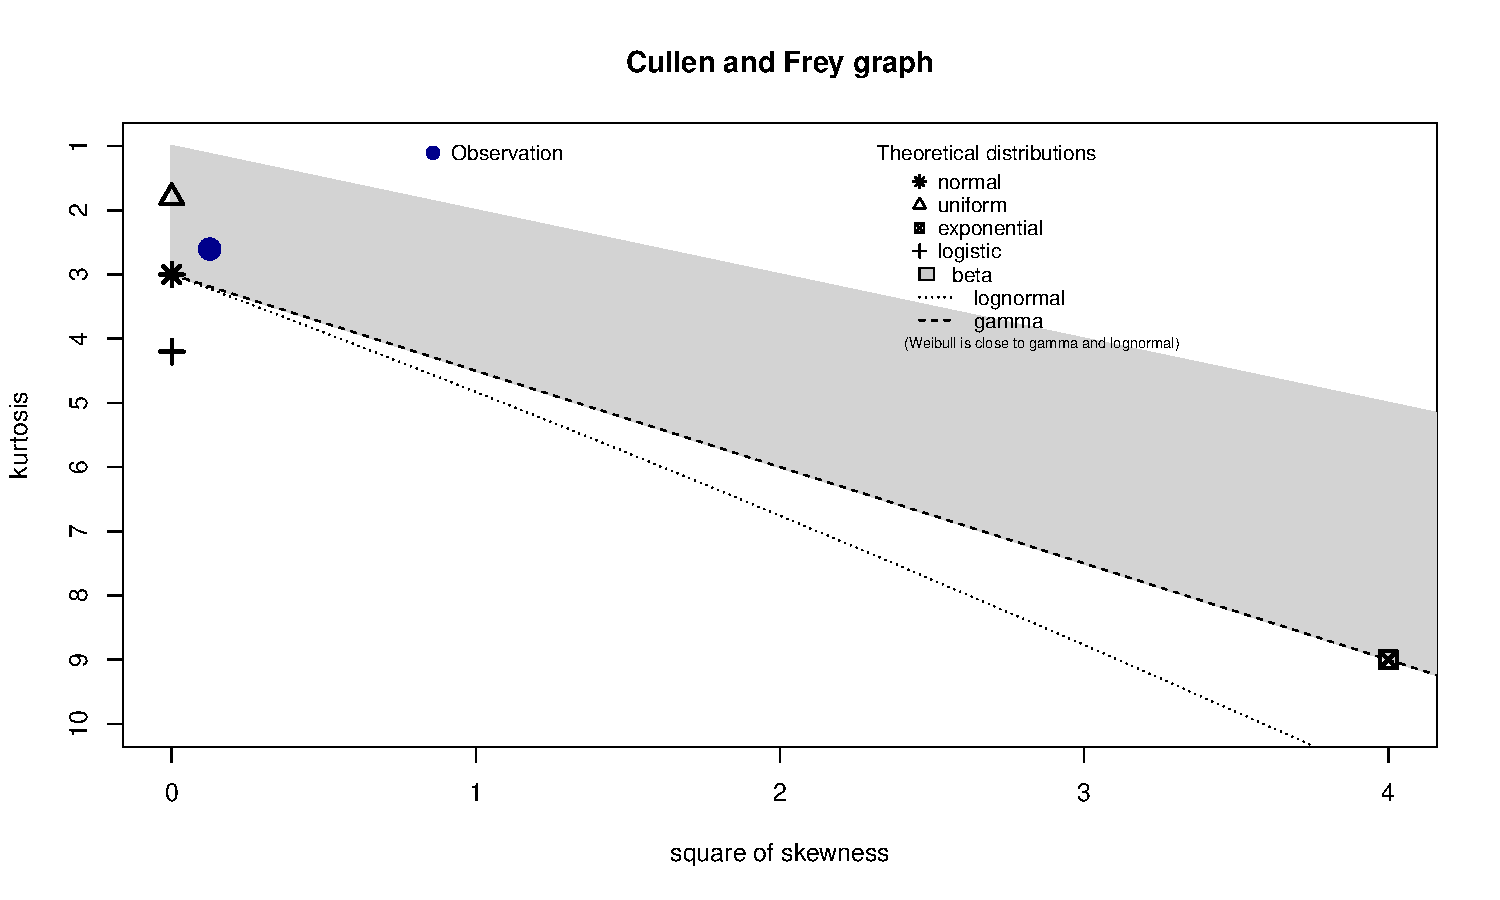
\includegraphics{Final_Project_files/figure-latex/unnamed-chunk-6-1.pdf}

\newpage

We can further see that Des Moines accounts for a significant portion of
the liquor sales in Polk County. Polk County is the most populous county
in Iowa so we will limit our analysis to this city.

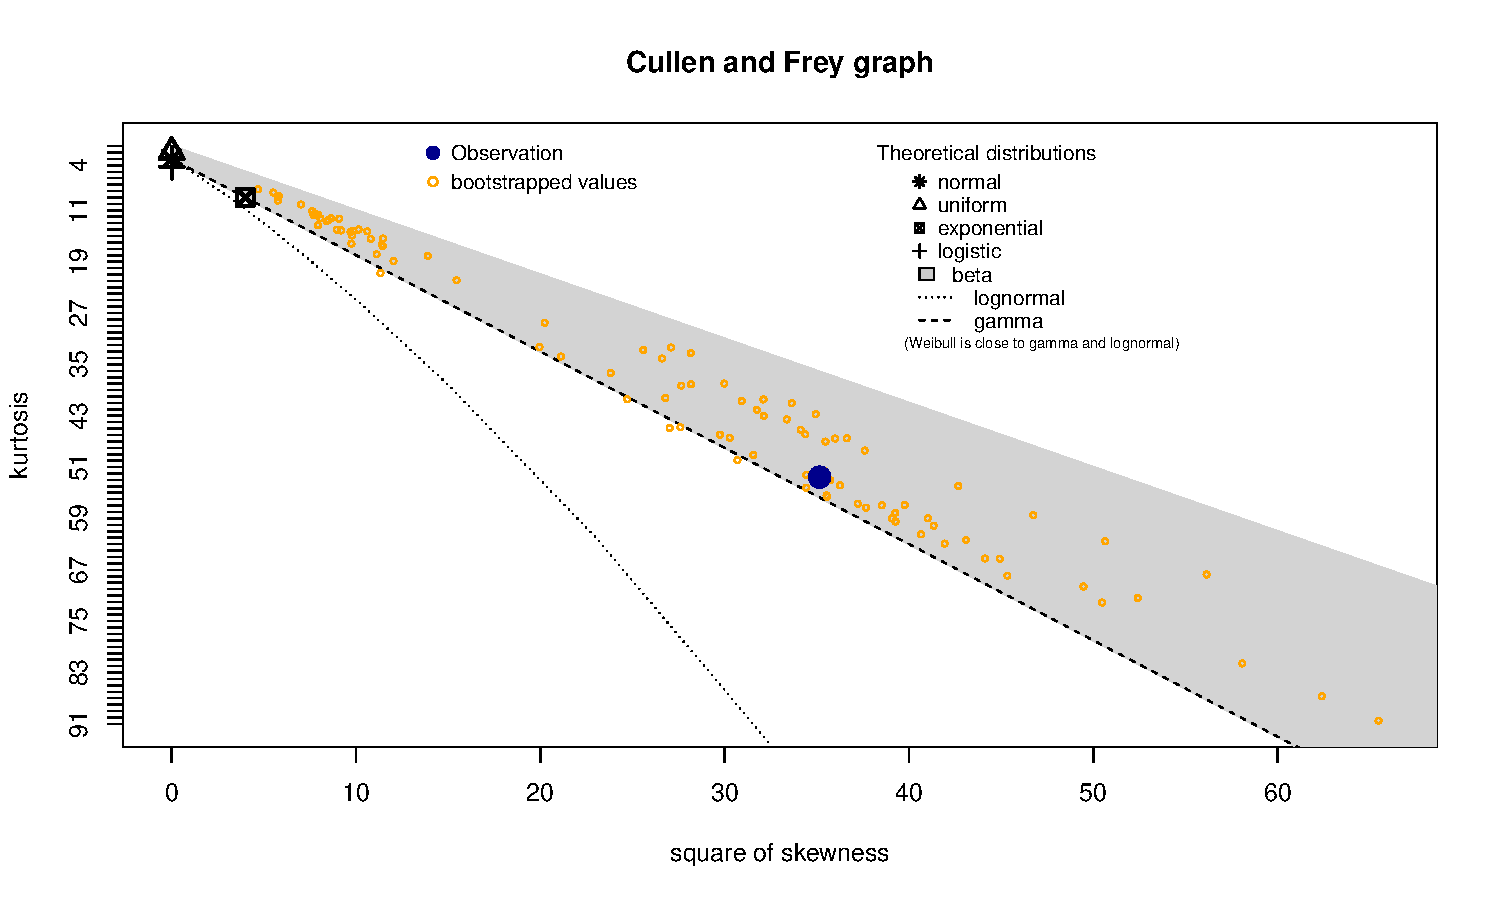
\includegraphics{Final_Project_files/figure-latex/unnamed-chunk-9-1.pdf}

\subsubsection{Model Development}\label{model-development}

\subsubsection{Bottles Sold Model}\label{bottles-sold-model}

We used forward selection method for our initial model for the Bottles
Sold. However, we expect some high degrees of multicollinearity as some
of our variables can be easily explained by other variables in the data
set. We see a very high degree of multicollinearity in our independent
variables for Bottles Sold and with good reason. If more bottles sold
then certainly the volume sold by gallons would increase as would the
sale dollars, we therefore removed volume sold by gallons. Below is the
table that highlights the high levels of multicollinearity for Volume
Sold by Gallons and Sale Dollars.

\begin{longtable}[]{@{}lcccc@{}}
\toprule
rn & GVIF & Df & GVIF\^{}(1/(2*Df)) & Adjusted\_GVIF\tabularnewline
\midrule
\endhead
Volume.Sold..Gallons. & 37.245911 & 1 & 6.102943 &
37.245911\tabularnewline
Category.Name & 1.738855 & 7 & 1.040307 & 1.082239\tabularnewline
State.Bottle.Retail & 2.359291 & 1 & 1.535998 & 2.359291\tabularnewline
Pack & 1.248515 & 1 & 1.117370 & 1.248515\tabularnewline
Sale..Dollars. & 33.330891 & 1 & 5.773291 & 33.330891\tabularnewline
\bottomrule
\end{longtable}

\subsubsection{Removing Influenctial
points}\label{removing-influenctial-points}

However, several values may have undue influence on the final form of
our model. Using the \texttt{influencePlot} function from the
\texttt{car} package and Cooks Distance plot, we can see which values
that have the greatest impact on our model and we removed the
observations indicated in the Cook's distance plot for 65, 70, and 227.
We do see that the influenceplot function indicated observation 74,
however, we chose to include this observation due to our comfort with
the Cook's distance plot from Base R which did not indicate the same
observation.

\begin{longtable}[]{@{}cccc@{}}
\caption{Influential points in Bottles Sold Model for influencePlot
function}\tabularnewline
\toprule
\begin{minipage}[b]{0.12\columnwidth}\centering\strut
~\strut
\end{minipage} & \begin{minipage}[b]{0.12\columnwidth}\centering\strut
StudRes\strut
\end{minipage} & \begin{minipage}[b]{0.10\columnwidth}\centering\strut
Hat\strut
\end{minipage} & \begin{minipage}[b]{0.10\columnwidth}\centering\strut
CookD\strut
\end{minipage}\tabularnewline
\midrule
\endfirsthead
\toprule
\begin{minipage}[b]{0.12\columnwidth}\centering\strut
~\strut
\end{minipage} & \begin{minipage}[b]{0.12\columnwidth}\centering\strut
StudRes\strut
\end{minipage} & \begin{minipage}[b]{0.10\columnwidth}\centering\strut
Hat\strut
\end{minipage} & \begin{minipage}[b]{0.10\columnwidth}\centering\strut
CookD\strut
\end{minipage}\tabularnewline
\midrule
\endhead
\begin{minipage}[t]{0.12\columnwidth}\centering\strut
\textbf{70}\strut
\end{minipage} & \begin{minipage}[t]{0.12\columnwidth}\centering\strut
-1.216\strut
\end{minipage} & \begin{minipage}[t]{0.10\columnwidth}\centering\strut
0.4126\strut
\end{minipage} & \begin{minipage}[t]{0.10\columnwidth}\centering\strut
0.09429\strut
\end{minipage}\tabularnewline
\begin{minipage}[t]{0.12\columnwidth}\centering\strut
\textbf{74}\strut
\end{minipage} & \begin{minipage}[t]{0.12\columnwidth}\centering\strut
7.415\strut
\end{minipage} & \begin{minipage}[t]{0.10\columnwidth}\centering\strut
0.01616\strut
\end{minipage} & \begin{minipage}[t]{0.10\columnwidth}\centering\strut
0.07151\strut
\end{minipage}\tabularnewline
\begin{minipage}[t]{0.12\columnwidth}\centering\strut
\textbf{227}\strut
\end{minipage} & \begin{minipage}[t]{0.12\columnwidth}\centering\strut
5.591\strut
\end{minipage} & \begin{minipage}[t]{0.10\columnwidth}\centering\strut
0.04581\strut
\end{minipage} & \begin{minipage}[t]{0.10\columnwidth}\centering\strut
0.126\strut
\end{minipage}\tabularnewline
\bottomrule
\end{longtable}

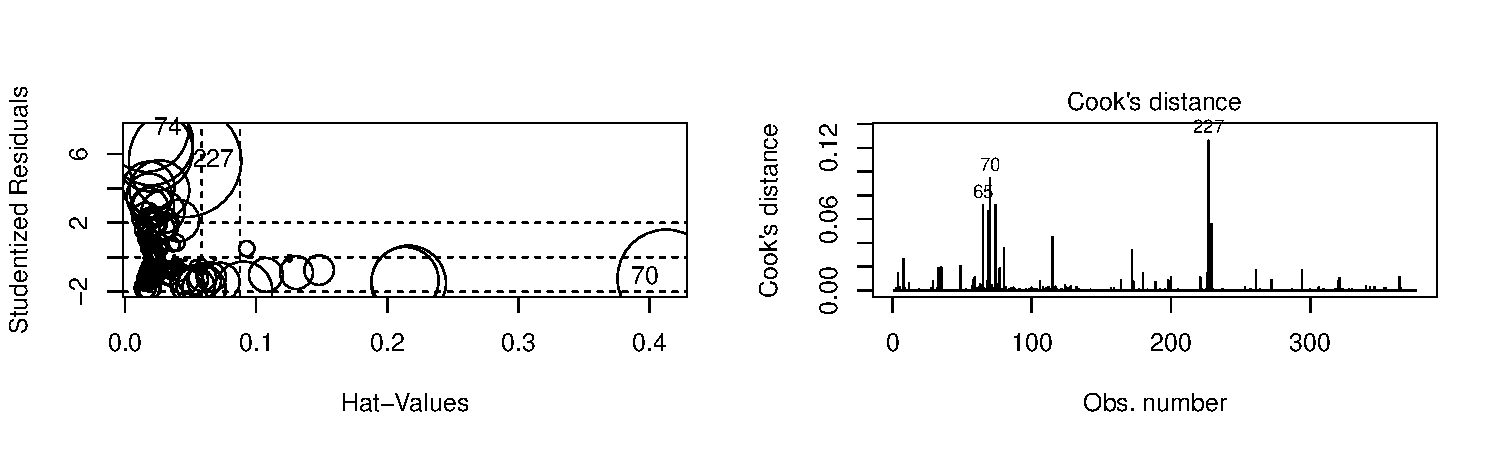
\includegraphics{Final_Project_files/figure-latex/unnamed-chunk-12-1.pdf}

\begin{table}[!htbp] \centering 
  \caption{Forward Selection Linear Model for Bottles Sold with Influencial Points} 
  \label{} 
\normalsize 
\begin{tabular}{@{\extracolsep{5pt}}lc} 
\\[-1.8ex]\hline 
\hline \\[-1.8ex] 
 & \multicolumn{1}{c}{\textit{Dependent variable:}} \\ 
\cline{2-2} 
\\[-1.8ex] & Bottles.Sold \\ 
\hline \\[-1.8ex] 
 Constant & $-$26.962$^{***}$ (7.283) \\ 
  Volume.Sold..Gallons. & 3.750$^{***}$ (0.040) \\ 
  Category.NameCANADIAN WHISKIES & 34.750$^{***}$ (6.600) \\ 
  Category.NameIRISH WHISKIES & $-$10.615 (7.679) \\ 
  Category.NameSCOTCH WHISKIES & $-$14.066$^{*}$ (7.765) \\ 
  Category.NameSINGLE BARREL BOURBON WHISKIES & 6.983 (14.477) \\ 
  Category.NameSTRAIGHT BOURBON WHISKIES & $-$7.049 (6.820) \\ 
  Category.NameSTRAIGHT RYE WHISKIES & 11.064 (9.070) \\ 
  Category.NameTENNESSEE WHISKIES & $-$6.569 (6.743) \\ 
  State.Bottle.Retail & 0.084$^{***}$ (0.011) \\ 
  Pack & 2.709$^{***}$ (0.368) \\ 
 \hline \\[-1.8ex] 
Observations & 376 \\ 
R$^{2}$ & 0.984 \\ 
Adjusted R$^{2}$ & 0.984 \\ 
Residual Std. Error & 37.354 (df = 365) \\ 
F Statistic & 2,259.802$^{***}$ (df = 10; 365)  (p = 0.000) \\ 
\hline 
\hline \\[-1.8ex] 
\textit{Note:}  & \multicolumn{1}{r}{$^{*}$p$<$0.1; $^{**}$p$<$0.05; $^{***}$p$<$0.01} \\ 
\end{tabular} 
\end{table}

Below are the diagnostic plots for our Model 1, without influential
points. Unfortunately, we see a non-normal distribution in residuals of
the qq plot and we see a linear relationship for the fitted and actual
values plot.

\begin{table}[!htbp] \centering 
  \caption{Forward Selection Linear Model for Bottles Sold without Influencial Points} 
  \label{} 
\normalsize 
\begin{tabular}{@{\extracolsep{5pt}}lc} 
\\[-1.8ex]\hline 
\hline \\[-1.8ex] 
 & \multicolumn{1}{c}{\textit{Dependent variable:}} \\ 
\cline{2-2} 
\\[-1.8ex] & Bottles.Sold \\ 
\hline \\[-1.8ex] 
 Constant & $-$25.596$^{***}$ (6.602) \\ 
  Volume.Sold..Gallons. & 3.771$^{***}$ (0.045) \\ 
  Category.NameCANADIAN WHISKIES & 32.910$^{***}$ (6.002) \\ 
  Category.NameIRISH WHISKIES & $-$10.398 (6.947) \\ 
  Category.NameSCOTCH WHISKIES & $-$12.880$^{*}$ (7.053) \\ 
  Category.NameSINGLE BARREL BOURBON WHISKIES & 6.909 (13.108) \\ 
  Category.NameSTRAIGHT BOURBON WHISKIES & $-$8.602 (6.185) \\ 
  Category.NameSTRAIGHT RYE WHISKIES & 10.806 (8.213) \\ 
  Category.NameTENNESSEE WHISKIES & $-$6.136 (6.102) \\ 
  State.Bottle.Retail & 0.072$^{***}$ (0.011) \\ 
  Pack & 2.647$^{***}$ (0.333) \\ 
 \hline \\[-1.8ex] 
Observations & 373 \\ 
R$^{2}$ & 0.981 \\ 
Adjusted R$^{2}$ & 0.980 \\ 
Residual Std. Error & 33.781 (df = 362) \\ 
F Statistic & 1,833.018$^{***}$ (df = 10; 362)  (p = 0.000) \\ 
\hline 
\hline \\[-1.8ex] 
\textit{Note:}  & \multicolumn{1}{r}{$^{*}$p$<$0.1; $^{**}$p$<$0.05; $^{***}$p$<$0.01} \\ 
\end{tabular} 
\end{table}

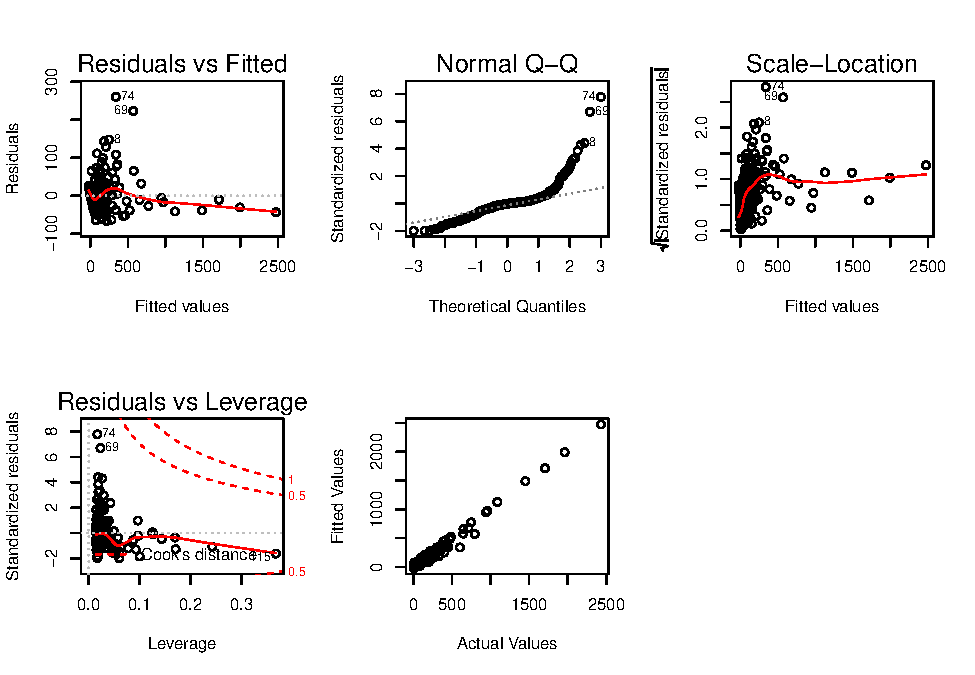
\includegraphics{Final_Project_files/figure-latex/unnamed-chunk-13-1.pdf}

Our model has an extremely good Adjusted \(R^2\) at 0.98 but we see that
the distribution of the residuals is not normally distributed and the
fitted values plotted to the actual values do show a clearly linear
relationship. We will need to further transform the variables in order
to have a more normal distribution of our residuals. We have an
interesting correlation in that an increase in the Retail Price will
have a .0723 increase in the number of bottles sold. The expectation
would be that as retail price increases the number of bottles sold would
decrease.

\subsubsection{Bottles Sold Model with Log
Transformation}\label{bottles-sold-model-with-log-transformation}

Our adjusted model uses the same selection method of forward and keeps
Bottles Sold as our dependent variable. However, we use the BoxCox
transformation method to transform our dependent variable. The resulting
\(\lambda\) is 0 so our transformation is log. In using this selection
method and dependent variable transformation, the final model excludes
the Sales Dollars variable. Additionally, we have high multicollinearity
between the Bottle Cost and the Retail variables, which is intuitive
because Bottle Cost has a high impact on Retail price. We remove the
Bottle Cost variable as we have more interest in the impacts Retail
Price may have on our dependent variable.

\begin{longtable}[]{@{}lcccc@{}}
\toprule
rn & GVIF & Df & GVIF\^{}(1/(2*Df)) & Adjusted\_GVIF\tabularnewline
\midrule
\endhead
State.Bottle.Cost & 5.159072e+05 & 1 & 718.266832 &
5.159072e+05\tabularnewline
Category.Name & 2.102294e+00 & 7 & 1.054507 &
1.111985e+00\tabularnewline
State.Bottle.Retail & 5.158069e+05 & 1 & 718.196947 &
5.158069e+05\tabularnewline
Pack & 2.516499e+00 & 1 & 1.586348 & 2.516499e+00\tabularnewline
Volume.Sold..Gallons. & 2.231722e+00 & 1 & 1.493895 &
2.231722e+00\tabularnewline
Bottle.Volume..ml. & 2.332312e+00 & 1 & 1.527191 &
2.332312e+00\tabularnewline
\bottomrule
\end{longtable}

\begin{table}[!htbp] \centering 
  \caption{Forward Selection Linear Model for Log Bottles Sold with Influencial Points} 
  \label{} 
\normalsize 
\begin{tabular}{@{\extracolsep{5pt}}lc} 
\\[-1.8ex]\hline 
\hline \\[-1.8ex] 
 & \multicolumn{1}{c}{\textit{Dependent variable:}} \\ 
\cline{2-2} 
\\[-1.8ex] & log(Bottles.Sold) \\ 
\hline \\[-1.8ex] 
 Constant & 1.845$^{***}$ (0.447) \\ 
  Category.NameCANADIAN WHISKIES & 0.730$^{***}$ (0.191) \\ 
  Category.NameIRISH WHISKIES & $-$0.761$^{***}$ (0.226) \\ 
  Category.NameSCOTCH WHISKIES & $-$0.680$^{***}$ (0.220) \\ 
  Category.NameSINGLE BARREL BOURBON WHISKIES & $-$1.062$^{**}$ (0.429) \\ 
  Category.NameSTRAIGHT BOURBON WHISKIES & $-$0.326 (0.202) \\ 
  Category.NameSTRAIGHT RYE WHISKIES & $-$0.649$^{**}$ (0.286) \\ 
  Category.NameTENNESSEE WHISKIES & $-$0.313 (0.198) \\ 
  State.Bottle.Retail & 0.003$^{***}$ (0.0003) \\ 
  Pack & 0.060$^{***}$ (0.014) \\ 
  Volume.Sold..Gallons. & 0.004$^{***}$ (0.001) \\ 
  Bottle.Volume..ml. & 0.001$^{**}$ (0.0002) \\ 
 \hline \\[-1.8ex] 
Observations & 376 \\ 
R$^{2}$ & 0.583 \\ 
Adjusted R$^{2}$ & 0.570 \\ 
Residual Std. Error & 1.032 (df = 364) \\ 
F Statistic & 46.203$^{***}$ (df = 11; 364)  (p = 0.000) \\ 
\hline 
\hline \\[-1.8ex] 
\textit{Note:}  & \multicolumn{1}{r}{$^{*}$p$<$0.1; $^{**}$p$<$0.05; $^{***}$p$<$0.01} \\ 
\end{tabular} 
\end{table}

We select the values that have the greatest influence on our model and
remove them to improve the model performance. The observations removed
in this model is 70, 229, 272. We excluded 272 as indicated in the
Cook's distance plot from Base R. By excluding these values from our
evaluation data set we are able to fit a more appropriate model.

\begin{longtable}[]{@{}cccc@{}}
\caption{Influential points in Log of Bottles Sold Model from
influencePlot function}\tabularnewline
\toprule
\begin{minipage}[b]{0.12\columnwidth}\centering\strut
~\strut
\end{minipage} & \begin{minipage}[b]{0.12\columnwidth}\centering\strut
StudRes\strut
\end{minipage} & \begin{minipage}[b]{0.09\columnwidth}\centering\strut
Hat\strut
\end{minipage} & \begin{minipage}[b]{0.09\columnwidth}\centering\strut
CookD\strut
\end{minipage}\tabularnewline
\midrule
\endfirsthead
\toprule
\begin{minipage}[b]{0.12\columnwidth}\centering\strut
~\strut
\end{minipage} & \begin{minipage}[b]{0.12\columnwidth}\centering\strut
StudRes\strut
\end{minipage} & \begin{minipage}[b]{0.09\columnwidth}\centering\strut
Hat\strut
\end{minipage} & \begin{minipage}[b]{0.09\columnwidth}\centering\strut
CookD\strut
\end{minipage}\tabularnewline
\midrule
\endhead
\begin{minipage}[t]{0.12\columnwidth}\centering\strut
\textbf{70}\strut
\end{minipage} & \begin{minipage}[t]{0.12\columnwidth}\centering\strut
-3.358\strut
\end{minipage} & \begin{minipage}[t]{0.09\columnwidth}\centering\strut
0.4135\strut
\end{minipage} & \begin{minipage}[t]{0.09\columnwidth}\centering\strut
0.6442\strut
\end{minipage}\tabularnewline
\begin{minipage}[t]{0.12\columnwidth}\centering\strut
\textbf{229}\strut
\end{minipage} & \begin{minipage}[t]{0.12\columnwidth}\centering\strut
-4.322\strut
\end{minipage} & \begin{minipage}[t]{0.09\columnwidth}\centering\strut
0.2167\strut
\end{minipage} & \begin{minipage}[t]{0.09\columnwidth}\centering\strut
0.4107\strut
\end{minipage}\tabularnewline
\bottomrule
\end{longtable}

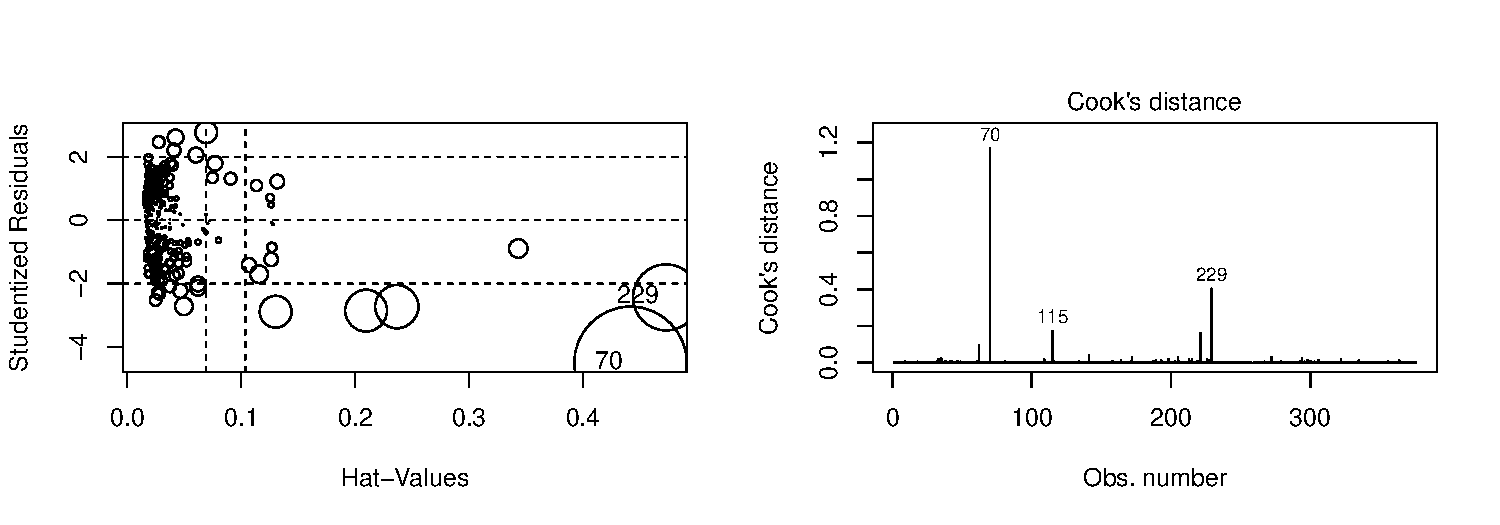
\includegraphics{Final_Project_files/figure-latex/unnamed-chunk-14-1.pdf}

\newpage

We further examine our diagnostic plots for our first model with the log
transformation.

\begin{table}[!htbp] \centering 
  \caption{Forward Selection Linear Model for Log of Bottles Sold without Influencial Points} 
  \label{} 
\normalsize 
\begin{tabular}{@{\extracolsep{5pt}}lc} 
\\[-1.8ex]\hline 
\hline \\[-1.8ex] 
 & \multicolumn{1}{c}{\textit{Dependent variable:}} \\ 
\cline{2-2} 
\\[-1.8ex] & log(Bottles.Sold) \\ 
\hline \\[-1.8ex] 
 Constant & 1.863$^{***}$ (0.414) \\ 
  Category.NameCANADIAN WHISKIES & 0.626$^{***}$ (0.178) \\ 
  Category.NameIRISH WHISKIES & $-$0.788$^{***}$ (0.209) \\ 
  Category.NameSCOTCH WHISKIES & $-$0.710$^{***}$ (0.205) \\ 
  Category.NameSINGLE BARREL BOURBON WHISKIES & $-$1.026$^{**}$ (0.398) \\ 
  Category.NameSTRAIGHT BOURBON WHISKIES & $-$0.279 (0.188) \\ 
  Category.NameSTRAIGHT RYE WHISKIES & $-$0.629$^{**}$ (0.265) \\ 
  Category.NameTENNESSEE WHISKIES & $-$0.336$^{*}$ (0.184) \\ 
  State.Bottle.Retail & 0.003$^{***}$ (0.0003) \\ 
  Pack & 0.058$^{***}$ (0.013) \\ 
  Volume.Sold..Gallons. & 0.008$^{***}$ (0.001) \\ 
  Bottle.Volume..ml. & 0.0005$^{**}$ (0.0002) \\ 
 \hline \\[-1.8ex] 
Observations & 373 \\ 
R$^{2}$ & 0.622 \\ 
Adjusted R$^{2}$ & 0.611 \\ 
Residual Std. Error & 0.957 (df = 361) \\ 
F Statistic & 54.043$^{***}$ (df = 11; 361)  (p = 0.000) \\ 
\hline 
\hline \\[-1.8ex] 
\textit{Note:}  & \multicolumn{1}{r}{$^{*}$p$<$0.1; $^{**}$p$<$0.05; $^{***}$p$<$0.01} \\ 
\end{tabular} 
\end{table}

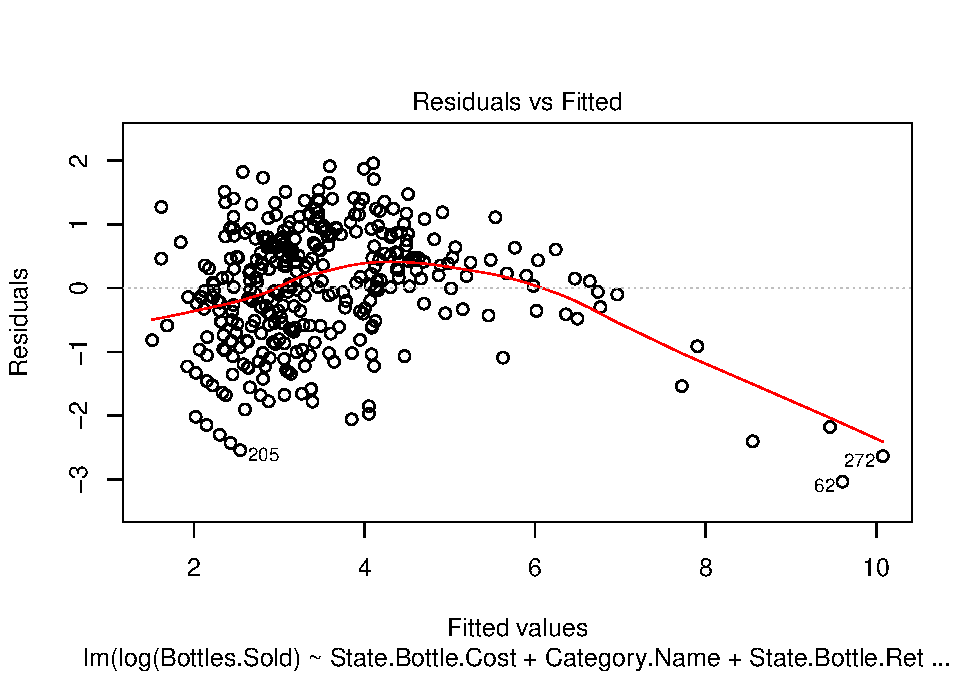
\includegraphics{Final_Project_files/figure-latex/unnamed-chunk-16-1.pdf}

\bigskip

The table of our detailed model is located in the Appendix and
fortunately, we see a much more normal distribution of the residuals.
Interestingly, our results show that one unit increase in the Retail
will increase the log of bottles sold by .0032 units. We would expect a
negative correlation with bottles price and bottles sold. Canadian
whiskies, Irish Whiskies, and Scotch were shown to be the most
significant but they do represent the majority of sales while Single
Barrel Bourbon Whiskies and Straight Rye Whiskies are approaching
significance. In comparison to Blended Whiskey, Canadian Whiskies will
increase the log of bottles sold by 0.62, whereas, Irish Whiskies will
decrease the log of bottles sold by 0.788 and Scotch will decrease the
log of bottles sold by 0.71.

Also, as expected, a unit increase in the Pack will increase the log of
bottles sold by 0.058 units. Another interesting finding is that a unit
increase in Bottle Volume will increase log of bottles sold by .0005
units, it would suggest that larger bottles are correlated with better
sales. The Adjusted R\^{}2 was improved from .588 to .631 by removing
the influence points. Also, the AIC of this model is 1039.469 which is a
much better AIC than 3697.202 from our non log previous model.

\newpage

\subsubsection{Profit Dollars Model
Development}\label{profit-dollars-model-development}

We now developed a model for the Profit Dollars for Whiskey sales in Des
Moines. Profit Dollars is measured as the Retail Sale less the Cost of
the liquor. We measure this value as pricing strategies are necessary in
attempting to maximize profit will maintaining efficient inventory
control. Using the forward selection method we find that the variables
\texttt{Pack} and \texttt{Bottle\ Volume\ in\ ml} are not significant so
they will be removed from our final model.

\begin{table}[!htbp] \centering 
  \caption{Forward Selection Linear Model for Profit Dollars with Influencial Points} 
  \label{} 
\normalsize 
\begin{tabular}{@{\extracolsep{5pt}}lc} 
\\[-1.8ex]\hline 
\hline \\[-1.8ex] 
 & \multicolumn{1}{c}{\textit{Dependent variable:}} \\ 
\cline{2-2} 
\\[-1.8ex] & ProfitDollar \\ 
\hline \\[-1.8ex] 
 Constant & $-$1.775 (8.092) \\ 
  Volume.Sold..Gallons. & 1.696$^{***}$ (0.238) \\ 
  Category.NameCANADIAN WHISKIES & 25.145$^{**}$ (10.301) \\ 
  Category.NameIRISH WHISKIES & 23.256$^{*}$ (12.611) \\ 
  Category.NameSCOTCH WHISKIES & 55.807$^{***}$ (12.373) \\ 
  Category.NameSINGLE BARREL BOURBON WHISKIES & 31.182 (22.246) \\ 
  Category.NameSTRAIGHT BOURBON WHISKIES & 54.113$^{***}$ (10.599) \\ 
  Category.NameSTRAIGHT RYE WHISKIES & 22.644 (14.061) \\ 
  Category.NameTENNESSEE WHISKIES & 24.333$^{**}$ (11.121) \\ 
  Sale..Dollars. & $-$0.009$^{***}$ (0.003) \\ 
 \hline \\[-1.8ex] 
Observations & 376 \\ 
R$^{2}$ & 0.575 \\ 
Adjusted R$^{2}$ & 0.565 \\ 
Residual Std. Error & 58.462 (df = 366) \\ 
F Statistic & 55.042$^{***}$ (df = 9; 366)  (p = 0.000) \\ 
\hline 
\hline \\[-1.8ex] 
\textit{Note:}  & \multicolumn{1}{r}{$^{*}$p$<$0.1; $^{**}$p$<$0.05; $^{***}$p$<$0.01} \\ 
\end{tabular} 
\end{table}

We further remove the influential points that are outliers as we did in
our previous model by the observations illustrated by our influence plot
and Cooks distance plot.

\begin{longtable}[]{@{}cccc@{}}
\caption{Influential points in Profit Dollars Model}\tabularnewline
\toprule
\begin{minipage}[b]{0.11\columnwidth}\centering\strut
~\strut
\end{minipage} & \begin{minipage}[b]{0.12\columnwidth}\centering\strut
StudRes\strut
\end{minipage} & \begin{minipage}[b]{0.09\columnwidth}\centering\strut
Hat\strut
\end{minipage} & \begin{minipage}[b]{0.09\columnwidth}\centering\strut
CookD\strut
\end{minipage}\tabularnewline
\midrule
\endfirsthead
\toprule
\begin{minipage}[b]{0.11\columnwidth}\centering\strut
~\strut
\end{minipage} & \begin{minipage}[b]{0.12\columnwidth}\centering\strut
StudRes\strut
\end{minipage} & \begin{minipage}[b]{0.09\columnwidth}\centering\strut
Hat\strut
\end{minipage} & \begin{minipage}[b]{0.09\columnwidth}\centering\strut
CookD\strut
\end{minipage}\tabularnewline
\midrule
\endhead
\begin{minipage}[t]{0.11\columnwidth}\centering\strut
\textbf{70}\strut
\end{minipage} & \begin{minipage}[t]{0.12\columnwidth}\centering\strut
-7.167\strut
\end{minipage} & \begin{minipage}[t]{0.09\columnwidth}\centering\strut
0.3365\strut
\end{minipage} & \begin{minipage}[t]{0.09\columnwidth}\centering\strut
2.29\strut
\end{minipage}\tabularnewline
\bottomrule
\end{longtable}

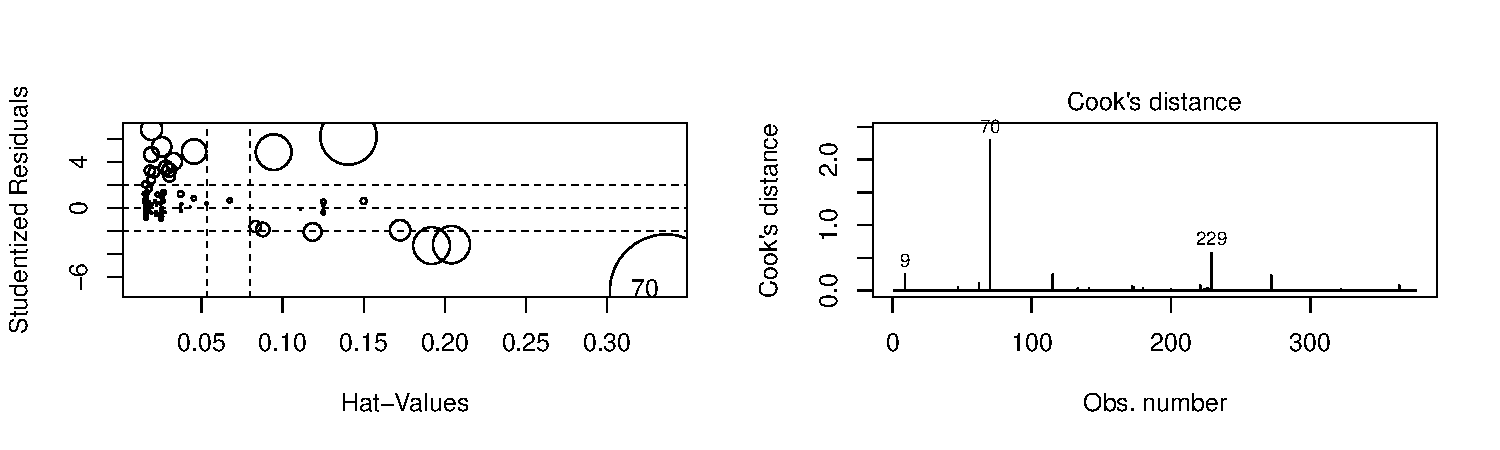
\includegraphics{Final_Project_files/figure-latex/unnamed-chunk-18-1.pdf}

\begin{table}[!htbp] \centering 
  \caption{Forward Selection Linear Model for Profit Dollars without Influencial Points} 
  \label{} 
\normalsize 
\begin{tabular}{@{\extracolsep{5pt}}lc} 
\\[-1.8ex]\hline 
\hline \\[-1.8ex] 
 & \multicolumn{1}{c}{\textit{Dependent variable:}} \\ 
\cline{2-2} 
\\[-1.8ex] & ProfitDollar \\ 
\hline \\[-1.8ex] 
 Constant & $-$2.458 (7.447) \\ 
  Volume.Sold..Gallons. & 1.680$^{***}$ (0.226) \\ 
  Category.NameCANADIAN WHISKIES & 27.875$^{***}$ (9.382) \\ 
  Category.NameIRISH WHISKIES & 21.716$^{*}$ (11.499) \\ 
  Category.NameSCOTCH WHISKIES & 54.760$^{***}$ (11.288) \\ 
  Category.NameSINGLE BARREL BOURBON WHISKIES & 31.538 (20.280) \\ 
  Category.NameSTRAIGHT BOURBON WHISKIES & 48.001$^{***}$ (9.705) \\ 
  Category.NameSTRAIGHT RYE WHISKIES & 22.161$^{*}$ (12.837) \\ 
  Category.NameTENNESSEE WHISKIES & 23.106$^{**}$ (10.147) \\ 
  Sale..Dollars. & $-$0.008$^{***}$ (0.002) \\ 
 \hline \\[-1.8ex] 
Observations & 374 \\ 
R$^{2}$ & 0.528 \\ 
Adjusted R$^{2}$ & 0.516 \\ 
Residual Std. Error & 53.219 (df = 364) \\ 
F Statistic & 45.190$^{***}$ (df = 9; 364)  (p = 0.000) \\ 
\hline 
\hline \\[-1.8ex] 
\textit{Note:}  & \multicolumn{1}{r}{$^{*}$p$<$0.1; $^{**}$p$<$0.05; $^{***}$p$<$0.01} \\ 
\end{tabular} 
\end{table}

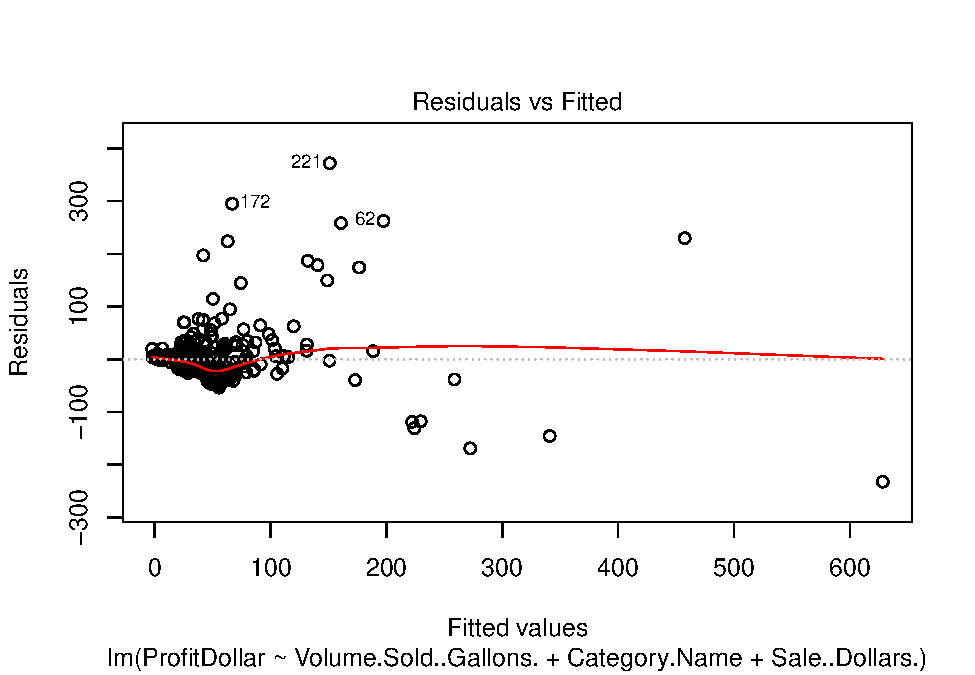
\includegraphics{Final_Project_files/figure-latex/unnamed-chunk-19-1.pdf}

Again, we see that the distribution of the residuals is not normally
distributed and the fitted values plotted to the actual values do show a
clearly linear relationship. We will need to further transform the
variables in order to have a more normal distribution of our residuals.
In performing a Box Cox transformation on the dependent variable we find
that the lambda value is close to 0 and we should therefore perform log
transformation.

\subsubsection{Profit Dollars Log Model}\label{profit-dollars-log-model}

The forward selection method removed the variable Pack from our final
model.

\begin{table}[!htbp] \centering 
  \caption{Forward Selection Linear Model for Log of Profit Dollars with Influencial Points} 
  \label{} 
\normalsize 
\begin{tabular}{@{\extracolsep{5pt}}lc} 
\\[-1.8ex]\hline 
\hline \\[-1.8ex] 
 & \multicolumn{1}{c}{\textit{Dependent variable:}} \\ 
\cline{2-2} 
\\[-1.8ex] & log(ProfitDollar) \\ 
\hline \\[-1.8ex] 
 Constant & 1.837$^{***}$ (0.208) \\ 
  Volume.Sold..Gallons. & 0.021$^{***}$ (0.004) \\ 
  Category.NameCANADIAN WHISKIES & 1.120$^{***}$ (0.174) \\ 
  Category.NameIRISH WHISKIES & 0.675$^{***}$ (0.212) \\ 
  Category.NameSCOTCH WHISKIES & 1.111$^{***}$ (0.205) \\ 
  Category.NameSINGLE BARREL BOURBON WHISKIES & 1.016$^{***}$ (0.369) \\ 
  Category.NameSTRAIGHT BOURBON WHISKIES & 0.833$^{***}$ (0.180) \\ 
  Category.NameSTRAIGHT RYE WHISKIES & 0.613$^{***}$ (0.235) \\ 
  Category.NameTENNESSEE WHISKIES & 0.916$^{***}$ (0.190) \\ 
  Sale..Dollars. & $-$0.0002$^{***}$ (0.00004) \\ 
  Bottle.Volume..ml. & 0.0004$^{**}$ (0.0002) \\ 
 \hline \\[-1.8ex] 
Observations & 376 \\ 
R$^{2}$ & 0.364 \\ 
Adjusted R$^{2}$ & 0.347 \\ 
Residual Std. Error & 0.966 (df = 365) \\ 
F Statistic & 20.901$^{***}$ (df = 10; 365)  (p = 0.000) \\ 
\hline 
\hline \\[-1.8ex] 
\textit{Note:}  & \multicolumn{1}{r}{$^{*}$p$<$0.1; $^{**}$p$<$0.05; $^{***}$p$<$0.01} \\ 
\end{tabular} 
\end{table}

We further remove the influential points that are outliers as we did in
our previous model by the observations illustrated by our influence plot
and Cooks distance plot.

\begin{longtable}[]{@{}cccc@{}}
\caption{Influential points in Log Profit Dollars Model from
influencePlot function}\tabularnewline
\toprule
\begin{minipage}[b]{0.11\columnwidth}\centering\strut
~\strut
\end{minipage} & \begin{minipage}[b]{0.12\columnwidth}\centering\strut
StudRes\strut
\end{minipage} & \begin{minipage}[b]{0.07\columnwidth}\centering\strut
Hat\strut
\end{minipage} & \begin{minipage}[b]{0.09\columnwidth}\centering\strut
CookD\strut
\end{minipage}\tabularnewline
\midrule
\endfirsthead
\toprule
\begin{minipage}[b]{0.11\columnwidth}\centering\strut
~\strut
\end{minipage} & \begin{minipage}[b]{0.12\columnwidth}\centering\strut
StudRes\strut
\end{minipage} & \begin{minipage}[b]{0.07\columnwidth}\centering\strut
Hat\strut
\end{minipage} & \begin{minipage}[b]{0.09\columnwidth}\centering\strut
CookD\strut
\end{minipage}\tabularnewline
\midrule
\endhead
\begin{minipage}[t]{0.11\columnwidth}\centering\strut
\textbf{70}\strut
\end{minipage} & \begin{minipage}[t]{0.12\columnwidth}\centering\strut
-5.123\strut
\end{minipage} & \begin{minipage}[t]{0.07\columnwidth}\centering\strut
0.338\strut
\end{minipage} & \begin{minipage}[t]{0.09\columnwidth}\centering\strut
1.14\strut
\end{minipage}\tabularnewline
\bottomrule
\end{longtable}

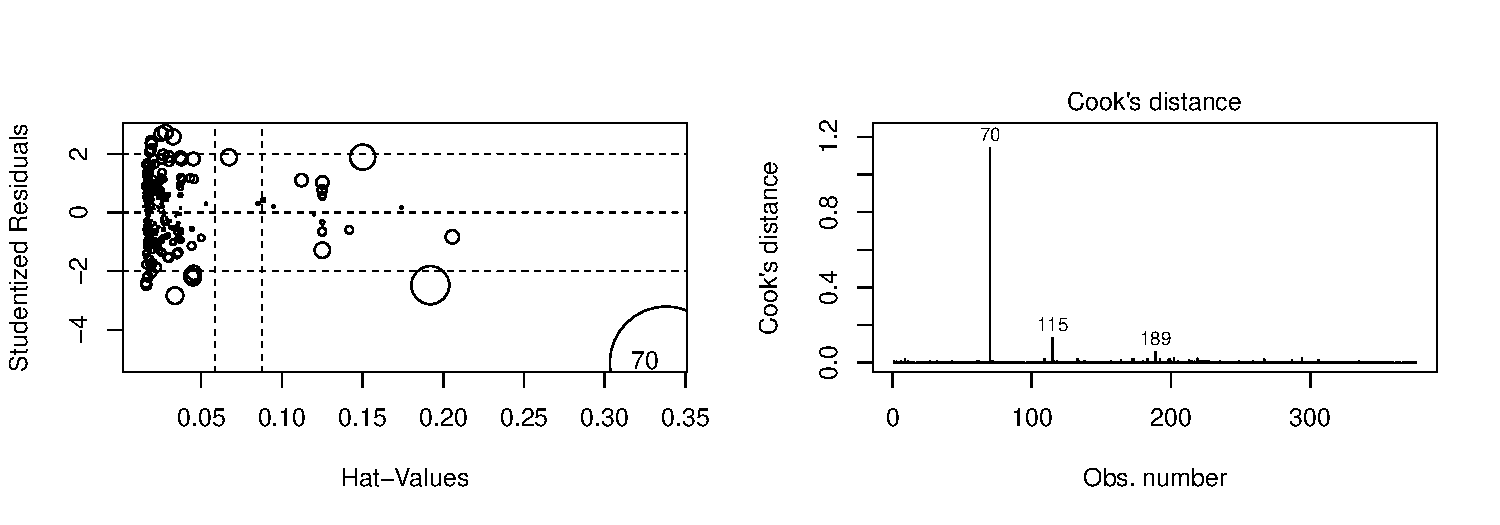
\includegraphics{Final_Project_files/figure-latex/unnamed-chunk-21-1.pdf}

\subsection{Diagnostic Plots}\label{diagnostic-plots}

\begin{table}[!htbp] \centering 
  \caption{Forward Selection Linear Model Log Profit Dollars without Influencial Points} 
  \label{} 
\normalsize 
\begin{tabular}{@{\extracolsep{5pt}}lc} 
\\[-1.8ex]\hline 
\hline \\[-1.8ex] 
 & \multicolumn{1}{c}{\textit{Dependent variable:}} \\ 
\cline{2-2} 
\\[-1.8ex] & log(ProfitDollar) \\ 
\hline \\[-1.8ex] 
 Constant & 1.777$^{***}$ (0.196) \\ 
  Volume.Sold..Gallons. & 0.028$^{***}$ (0.004) \\ 
  Category.NameCANADIAN WHISKIES & 1.171$^{***}$ (0.164) \\ 
  Category.NameIRISH WHISKIES & 0.707$^{***}$ (0.200) \\ 
  Category.NameSCOTCH WHISKIES & 1.133$^{***}$ (0.192) \\ 
  Category.NameSINGLE BARREL BOURBON WHISKIES & 1.120$^{***}$ (0.347) \\ 
  Category.NameSTRAIGHT BOURBON WHISKIES & 0.797$^{***}$ (0.169) \\ 
  Category.NameSTRAIGHT RYE WHISKIES & 0.694$^{***}$ (0.222) \\ 
  Category.NameTENNESSEE WHISKIES & 0.950$^{***}$ (0.180) \\ 
  Sale..Dollars. & $-$0.0002$^{***}$ (0.00004) \\ 
  Bottle.Volume..ml. & 0.0004$^{**}$ (0.0002) \\ 
 \hline \\[-1.8ex] 
Observations & 373 \\ 
R$^{2}$ & 0.426 \\ 
Adjusted R$^{2}$ & 0.410 \\ 
Residual Std. Error & 0.906 (df = 362) \\ 
F Statistic & 26.827$^{***}$ (df = 10; 362)  (p = 0.000) \\ 
\hline 
\hline \\[-1.8ex] 
\textit{Note:}  & \multicolumn{1}{r}{$^{*}$p$<$0.1; $^{**}$p$<$0.05; $^{***}$p$<$0.01} \\ 
\end{tabular} 
\end{table}

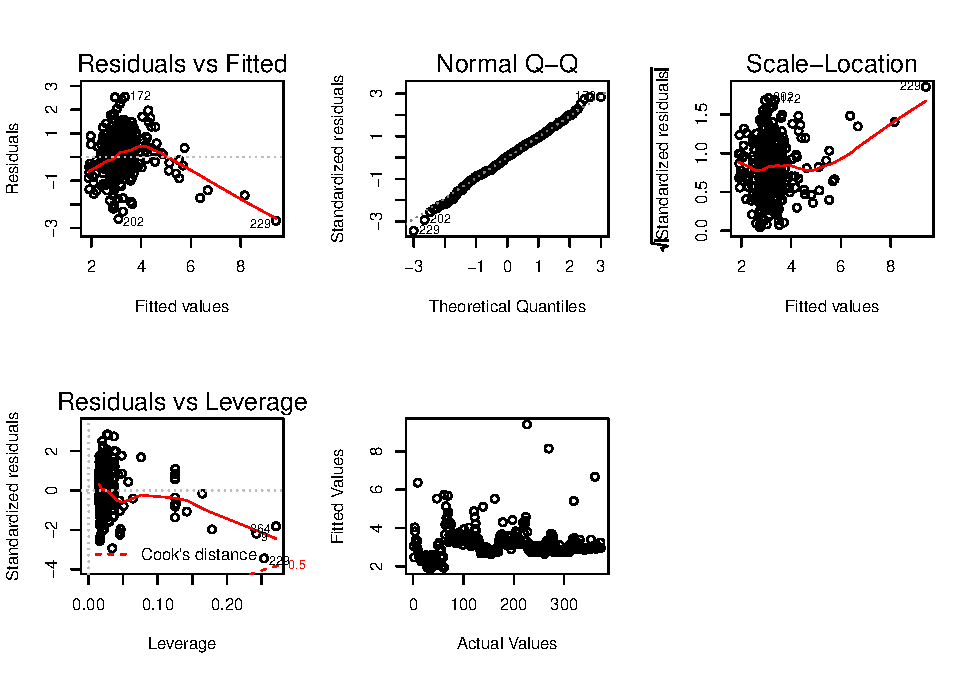
\includegraphics{Final_Project_files/figure-latex/unnamed-chunk-22-1.pdf}

The table of our detailed model for log Profit Dollars is located in the
Appendix and fortunately, we see a much more normal distribution of the
residuals. Interestingly, our results show that one unit increase in the
Bottle Volume will increase the log of Profit dollars by .0004 units. In
this model all Whiskies were shown to be significant and in comparison
to Blended Whiskey, Canadian Whiskies will increase the log of Profit
Dollars by 1.171, whereas, Irish Whiskies will only increase the log of
profit dollars by .707. None of the whiskies will reduce the log of
profit dollars.

Also, unexpectedly, a unit increase in the Sale Dollars will decrease
the log of profit dollars by 0.05 units. This is intuitive however,
because to increase sales we may have to reduce retail price and
therefore reduce our profit dollars. The Adjusted R\^{}2 for this model
was increased from .347 to .410 by removing the influencial points.
Also, the AIC of this model is 997.746 which is a much better than the
AIC of the non log transformed model at 4046.086.

\section{Discussion and Conclusions}\label{discussion-and-conclusions}

The resulting models allow us to model for November in Des Moines for
both Bottles Sold and Profit Dollars. We can utilize a naive forecast,
assuming that the prior year of 2015 is predictive of the year 2016.
However, there are further analysis types that may result in more robust
predictions.

In one study involving pharmaceutical distribution companies, the
purpose was to propose a novel method to forecast the sales of the
companies. Network-based analysis was conducted to find clique sets and
group members and to use the sales data of comembers. The reason for
this was the lack of sufficient historic sales records of each drug
(Neda Khalil Zadeh and Farvaresh (2014))

Three methods were used to build time series models forecasting sales -
ARIMA methodology, neural network, and an advanced hybrid neural network
approach. The performance of the proposed method was evaluated using a
real data set provided by one of the leading pharmacy distribution
companies in Iran. The results of the evaluation indicated that the
proposed method can cope with the low number of past records while
accurately forecasting medicine sales. An evaluation of the liquor data
set using these techniques may provide greater insight as the vast
number of records could produce a more accurate model (Neda Khalil Zadeh
and Farvaresh (2014)).

After exploratory analysis was done on the data, it was concluded that
most medicines had different and specific characteristics and sales
behavior, it was impractical to make a single prediction model for all
medicines, and most sales records had nonlinear relationships. This may
suggest that it would be more beneficial to model liquor categories
individually. However, the reason why the hybrid neural network method
was carried out was due to the fact that it is not acceptable to apply a
fully linear or nonlinear model on sales data. The two forecast error
measures that were used to evaluate and compare model performance were
mean squared error and mean absolute error. The performance of the
predicted data was significantly improved when the past records of
comembers were used (Neda Khalil Zadeh and Farvaresh (2014)).

In the other study that examined prediction-based inventory optimization
using data mining models, the Back propagation neural network method was
used for training the prediction model. The idea that gave rise to this
method of inventory prediction was the idea that the demand of marketing
is viewed as the foundation of inventory management. On the basis of the
prediction result, a simple and concise inventory policy was
established. Following this, the historic sales data was used to
estimate a normal distribution of demand and to calculate the inventory
cost with inventory strategy (Xiaoxiao Guo (2014)).

Two models (back propagation neural network and support vector
regression) were established using three input variables (historical
sales data, the frequency of searching the commodity, and the click
volume of the commodity page). When the back-propagation neural network
method was used, there was more accuracy shown in the performance
because the predicted values almost matched the actual values in the
graphs(Xiaoxiao Guo (2014)). This suggests that our naive forecast
approach could be improved through the use of these techniques in
conjunction with historical sales to create a more robust model.

In another study conducted in 2012 in Idaho, the monthly revenue
generated was examined rather than the yearly revenue generated which is
in line with our model approach for using a single month rather than a
year. The continued growth was rather owed to the number of weekends in
a month (five instead of four) and to the higher prices in neighboring
states. In Washington, the voters approved an initiative that led the
state to sell its liquor stores and add new distributor and retail fees,
making prices in the neighboring states (Idaho and Oregon) look better.
There were no changes made in marketing or pricing in response to the
regulatory shift in Washington (Iverson-Long (2012)). Further research
into the proximity of our counties to states and towns with higher
prices and regulation may provide more insight into bottles sold and
profit dollars. Additionally, reviewing the data by identifying months
that have five weekends instead of four could provide further insights.
A follow up study on how prices may have been impacted by pricing
strategies in neighboring states and the number of weekends per month
may offer further insights and improve the approach taken in this
analysis.

\newpage

\section{Appendices}\label{appendices}

\section{AIC Value Comparison}\label{aic-value-comparison}

\begin{longtable}[]{@{}cc@{}}
\caption{AIC Values}\tabularnewline
\toprule
\begin{minipage}[b]{0.29\columnwidth}\centering\strut
Model Name\strut
\end{minipage} & \begin{minipage}[b]{0.10\columnwidth}\centering\strut
AIC\strut
\end{minipage}\tabularnewline
\midrule
\endfirsthead
\toprule
\begin{minipage}[b]{0.29\columnwidth}\centering\strut
Model Name\strut
\end{minipage} & \begin{minipage}[b]{0.10\columnwidth}\centering\strut
AIC\strut
\end{minipage}\tabularnewline
\midrule
\endhead
\begin{minipage}[t]{0.29\columnwidth}\centering\strut
Bottles Sold\strut
\end{minipage} & \begin{minipage}[t]{0.10\columnwidth}\centering\strut
3697.202\strut
\end{minipage}\tabularnewline
\begin{minipage}[t]{0.29\columnwidth}\centering\strut
Log Bottles Sold\strut
\end{minipage} & \begin{minipage}[t]{0.10\columnwidth}\centering\strut
1039.469\strut
\end{minipage}\tabularnewline
\begin{minipage}[t]{0.29\columnwidth}\centering\strut
Profit Dollars\strut
\end{minipage} & \begin{minipage}[t]{0.10\columnwidth}\centering\strut
4046.086\strut
\end{minipage}\tabularnewline
\begin{minipage}[t]{0.29\columnwidth}\centering\strut
Log of Profit Dollars\strut
\end{minipage} & \begin{minipage}[t]{0.10\columnwidth}\centering\strut
997.746\strut
\end{minipage}\tabularnewline
\bottomrule
\end{longtable}

\section{Supplemental tables and
figures.}\label{supplemental-tables-and-figures.}

\begin{spacing}{0.7}
\begin{center}\textbf{ dfLiquorSales \\ 14 Variables~~~~~ 376 ~Observations}\end{center}
\smallskip\hrule\smallskip{\small
\noindent\textbf{Month}

{\smaller
\begin{tabular}{ rrrrrr }
n&missing&distinct&Info&Mean&Gmd \\
376&0&1&0&11&0 \end{tabular}
\begin{verbatim}
              
Value       11
Frequency  376
Proportion   1
\end{verbatim}
}
\smallskip\hrule\smallskip
\noindent\textbf{Year}

{\smaller
\begin{tabular}{ rrrrrr }
n&missing&distinct&Info&Mean&Gmd \\
376&0&1&0&2015&0 \end{tabular}
\begin{verbatim}
               
Value      2015
Frequency   376
Proportion    1
\end{verbatim}
}
\smallskip\hrule\smallskip
\noindent\textbf{City}

{\smaller
\begin{tabular}{ rrrr }
n&missing&distinct&value \\
376&0&1&DES MOINES \end{tabular}
\begin{verbatim}
                     
Value      DES MOINES
Frequency         376
Proportion          1
\end{verbatim}
}
\smallskip\hrule\smallskip
\noindent\textbf{Category.Name}\setlength{\unitlength}{0.001in}\hfill\begin{picture}(1.5,.1)(1500,0)\linethickness{0.6pt}
\put(0,0){\line(0,1){86}}
\put(188,0){\line(0,1){100}}
\put(375,0){\line(0,1){55}}
\put(562,0){\line(0,1){58}}
\put(750,0){\line(0,1){11}}
\put(938,0){\line(0,1){93}}
\put(1125,0){\line(0,1){38}}
\put(1312,0){\line(0,1){89}}
\end{picture}

{\smaller
\begin{tabular}{ rrr }
n&missing&distinct \\
376&0&8 \end{tabular}
\begin{verbatim}

BLENDED WHISKIES (61, 0.162), CANADIAN WHISKIES (71, 0.189), IRISH WHISKIES (39, 0.104),
SCOTCH WHISKIES (41, 0.109), SINGLE BARREL BOURBON WHISKIES (8, 0.021), STRAIGHT BOURBON
WHISKIES (66, 0.176), STRAIGHT RYE WHISKIES (27, 0.072), TENNESSEE WHISKIES (63, 0.168)
\end{verbatim}
}
\smallskip\hrule\smallskip
\noindent\textbf{Store.Number}\setlength{\unitlength}{0.001in}\hfill\begin{picture}(1.5,.1)(1500,0)\linethickness{0.6pt}
\put(0,0){\line(0,1){100}}
\put(29,0){\line(0,1){100}}
\put(167,0){\line(0,1){100}}
\put(168,0){\line(0,1){88}}
\put(170,0){\line(0,1){88}}
\put(184,0){\line(0,1){100}}
\put(217,0){\line(0,1){100}}
\put(217,0){\line(0,1){75}}
\put(220,0){\line(0,1){100}}
\put(221,0){\line(0,1){88}}
\put(328,0){\line(0,1){25}}
\put(329,0){\line(0,1){62}}
\put(601,0){\line(0,1){75}}
\put(739,0){\line(0,1){88}}
\put(748,0){\line(0,1){75}}
\put(786,0){\line(0,1){50}}
\put(789,0){\line(0,1){62}}
\put(792,0){\line(0,1){75}}
\put(812,0){\line(0,1){75}}
\put(838,0){\line(0,1){62}}
\put(927,0){\line(0,1){88}}
\put(930,0){\line(0,1){75}}
\put(968,0){\line(0,1){75}}
\put(969,0){\line(0,1){75}}
\put(983,0){\line(0,1){38}}
\put(991,0){\line(0,1){75}}
\put(1034,0){\line(0,1){75}}
\put(1045,0){\line(0,1){62}}
\put(1048,0){\line(0,1){38}}
\put(1069,0){\line(0,1){50}}
\put(1078,0){\line(0,1){62}}
\put(1086,0){\line(0,1){50}}
\put(1136,0){\line(0,1){75}}
\put(1153,0){\line(0,1){75}}
\put(1194,0){\line(0,1){50}}
\put(1194,0){\line(0,1){50}}
\put(1195,0){\line(0,1){50}}
\put(1195,0){\line(0,1){50}}
\put(1196,0){\line(0,1){25}}
\put(1196,0){\line(0,1){50}}
\put(1197,0){\line(0,1){50}}
\put(1197,0){\line(0,1){38}}
\put(1198,0){\line(0,1){38}}
\put(1205,0){\line(0,1){75}}
\put(1208,0){\line(0,1){38}}
\put(1217,0){\line(0,1){50}}
\put(1231,0){\line(0,1){50}}
\put(1294,0){\line(0,1){62}}
\put(1294,0){\line(0,1){62}}
\put(1296,0){\line(0,1){38}}
\put(1296,0){\line(0,1){38}}
\put(1297,0){\line(0,1){62}}
\put(1297,0){\line(0,1){88}}
\put(1298,0){\line(0,1){50}}
\put(1298,0){\line(0,1){50}}
\put(1311,0){\line(0,1){100}}
\put(1321,0){\line(0,1){25}}
\put(1359,0){\line(0,1){25}}
\put(1367,0){\line(0,1){38}}
\put(1383,0){\line(0,1){38}}
\put(1394,0){\line(0,1){88}}
\put(1421,0){\line(0,1){50}}
\put(1424,0){\line(0,1){62}}
\put(1458,0){\line(0,1){75}}
\put(1458,0){\line(0,1){88}}
\put(1459,0){\line(0,1){88}}
\put(1459,0){\line(0,1){88}}
\put(1460,0){\line(0,1){88}}
\put(1461,0){\line(0,1){62}}
\put(1461,0){\line(0,1){62}}
\put(1464,0){\line(0,1){38}}
\put(1468,0){\line(0,1){75}}
\put(1479,0){\line(0,1){50}}
\end{picture}

{\smaller
\begin{tabular}{ rrr }
n&missing&distinct \\
376&0&73 \end{tabular}
\begin{verbatim}

lowest : 2190 2248 2527 2528 2532, highest: 5131 5132 5137 5145 5169
\end{verbatim}
}
\smallskip\hrule\smallskip
\noindent\textbf{Store.Name}\setlength{\unitlength}{0.001in}\hfill\begin{picture}(1.5,.1)(1500,0)\linethickness{0.6pt}
\put(0,0){\line(0,1){44}}
\put(21,0){\line(0,1){44}}
\put(42,0){\line(0,1){22}}
\put(62,0){\line(0,1){67}}
\put(83,0){\line(0,1){78}}
\put(104,0){\line(0,1){89}}
\put(125,0){\line(0,1){89}}
\put(146,0){\line(0,1){22}}
\put(167,0){\line(0,1){56}}
\put(188,0){\line(0,1){78}}
\put(208,0){\line(0,1){33}}
\put(229,0){\line(0,1){56}}
\put(250,0){\line(0,1){67}}
\put(271,0){\line(0,1){67}}
\put(292,0){\line(0,1){22}}
\put(312,0){\line(0,1){67}}
\put(333,0){\line(0,1){67}}
\put(354,0){\line(0,1){89}}
\put(375,0){\line(0,1){89}}
\put(396,0){\line(0,1){78}}
\put(417,0){\line(0,1){78}}
\put(438,0){\line(0,1){89}}
\put(458,0){\line(0,1){89}}
\put(479,0){\line(0,1){67}}
\put(500,0){\line(0,1){78}}
\put(521,0){\line(0,1){89}}
\put(542,0){\line(0,1){44}}
\put(562,0){\line(0,1){33}}
\put(583,0){\line(0,1){33}}
\put(604,0){\line(0,1){56}}
\put(625,0){\line(0,1){44}}
\put(646,0){\line(0,1){67}}
\put(667,0){\line(0,1){67}}
\put(688,0){\line(0,1){56}}
\put(708,0){\line(0,1){100}}
\put(729,0){\line(0,1){56}}
\put(750,0){\line(0,1){78}}
\put(771,0){\line(0,1){78}}
\put(792,0){\line(0,1){78}}
\put(812,0){\line(0,1){44}}
\put(833,0){\line(0,1){22}}
\put(854,0){\line(0,1){44}}
\put(875,0){\line(0,1){44}}
\put(896,0){\line(0,1){56}}
\put(917,0){\line(0,1){33}}
\put(938,0){\line(0,1){44}}
\put(958,0){\line(0,1){44}}
\put(979,0){\line(0,1){44}}
\put(1000,0){\line(0,1){33}}
\put(1021,0){\line(0,1){33}}
\put(1042,0){\line(0,1){44}}
\put(1062,0){\line(0,1){67}}
\put(1083,0){\line(0,1){78}}
\put(1104,0){\line(0,1){67}}
\put(1125,0){\line(0,1){67}}
\put(1146,0){\line(0,1){67}}
\put(1167,0){\line(0,1){67}}
\put(1188,0){\line(0,1){33}}
\put(1208,0){\line(0,1){33}}
\put(1229,0){\line(0,1){56}}
\put(1250,0){\line(0,1){78}}
\put(1271,0){\line(0,1){67}}
\put(1292,0){\line(0,1){44}}
\put(1312,0){\line(0,1){67}}
\put(1333,0){\line(0,1){56}}
\put(1354,0){\line(0,1){56}}
\put(1375,0){\line(0,1){33}}
\put(1396,0){\line(0,1){56}}
\put(1417,0){\line(0,1){78}}
\put(1438,0){\line(0,1){44}}
\put(1458,0){\line(0,1){44}}
\put(1479,0){\line(0,1){33}}
\end{picture}

{\smaller
\begin{tabular}{ rrr }
n&missing&distinct \\
376&0&72 \end{tabular}
\begin{verbatim}

lowest : AV Superstop                  Best Food Mart / Des Moines   C Fresh Market                Cash Saver  /  E Euclid Ave   Cash Saver  /  Fleur         
highest: Walgreens #05852 / Des Moines Walgreens #07452 / Des Moines Walgreens #07453 / Des Moines Walgreens #07833 / Des Moines Walgreens #07968 / Des Moines
\end{verbatim}
}
\smallskip\hrule\smallskip
\noindent\textbf{Pack}\setlength{\unitlength}{0.001in}\hfill\begin{picture}(1.5,.1)(1500,0)\linethickness{0.6pt}
\put(0,0){\line(0,1){1}}
\put(67,0){\line(0,1){4}}
\put(89,0){\line(0,1){2}}
\put(111,0){\line(0,1){1}}
\put(134,0){\line(0,1){52}}
\put(178,0){\line(0,1){5}}
\put(200,0){\line(0,1){2}}
\put(223,0){\line(0,1){1}}
\put(245,0){\line(0,1){8}}
\put(267,0){\line(0,1){24}}
\put(290,0){\line(0,1){14}}
\put(312,0){\line(0,1){19}}
\put(334,0){\line(0,1){14}}
\put(356,0){\line(0,1){16}}
\put(379,0){\line(0,1){12}}
\put(401,0){\line(0,1){100}}
\put(423,0){\line(0,1){6}}
\put(445,0){\line(0,1){15}}
\put(468,0){\line(0,1){9}}
\put(490,0){\line(0,1){11}}
\put(512,0){\line(0,1){9}}
\put(535,0){\line(0,1){9}}
\put(557,0){\line(0,1){9}}
\put(579,0){\line(0,1){16}}
\put(601,0){\line(0,1){6}}
\put(624,0){\line(0,1){6}}
\put(646,0){\line(0,1){2}}
\put(668,0){\line(0,1){19}}
\put(690,0){\line(0,1){5}}
\put(713,0){\line(0,1){2}}
\put(735,0){\line(0,1){2}}
\put(757,0){\line(0,1){9}}
\put(780,0){\line(0,1){4}}
\put(802,0){\line(0,1){4}}
\put(824,0){\line(0,1){6}}
\put(846,0){\line(0,1){4}}
\put(869,0){\line(0,1){1}}
\put(891,0){\line(0,1){1}}
\put(935,0){\line(0,1){16}}
\put(1002,0){\line(0,1){2}}
\put(1025,0){\line(0,1){1}}
\put(1069,0){\line(0,1){2}}
\put(1091,0){\line(0,1){1}}
\put(1114,0){\line(0,1){4}}
\put(1136,0){\line(0,1){1}}
\put(1203,0){\line(0,1){1}}
\put(1292,0){\line(0,1){1}}
\put(1314,0){\line(0,1){1}}
\put(1381,0){\line(0,1){1}}
\put(1470,0){\line(0,1){4}}
\end{picture}

{\smaller
\begin{tabular}{ rrrrrrrrrrrrr }
n&missing&distinct&Info&Mean&Gmd&.05&.10&.25&.50&.75&.90&.95 \\
376&0&141&0.99&13.38&6.201& 6.00& 6.00& 9.75&12.00&16.00&21.37&24.00 \end{tabular}
\begin{verbatim}

lowest :  3.00000  4.50000  5.00000  5.25000  5.40000, highest: 30.00000 32.00000 32.57143 33.81818 36.00000
\end{verbatim}
}
\smallskip\hrule\smallskip
\noindent\textbf{Bottles.Sold}\setlength{\unitlength}{0.001in}\hfill\begin{picture}(1.5,.1)(1500,0)\linethickness{0.6pt}
\put(0,0){\line(0,1){100}}
\put(22,0){\line(0,1){46}}
\put(44,0){\line(0,1){23}}
\put(66,0){\line(0,1){15}}
\put(88,0){\line(0,1){7}}
\put(111,0){\line(0,1){3}}
\put(133,0){\line(0,1){2}}
\put(155,0){\line(0,1){3}}
\put(177,0){\line(0,1){2}}
\put(199,0){\line(0,1){2}}
\put(221,0){\line(0,1){1}}
\put(265,0){\line(0,1){1}}
\put(288,0){\line(0,1){1}}
\put(310,0){\line(0,1){1}}
\put(332,0){\line(0,1){1}}
\put(354,0){\line(0,1){1}}
\put(376,0){\line(0,1){1}}
\put(420,0){\line(0,1){1}}
\put(487,0){\line(0,1){1}}
\put(641,0){\line(0,1){1}}
\put(752,0){\line(0,1){1}}
\put(862,0){\line(0,1){1}}
\put(1084,0){\line(0,1){1}}
\put(1438,0){\line(0,1){1}}
\end{picture}

{\smaller[2]
\begin{tabular}{ rrrrrrrrrrrrr }
n&missing&distinct&Info&Mean&Gmd&.05&.10&.25&.50&.75&.90&.95 \\
376&0&153&0.999&116.1&173.3&  3.00&  5.00&  9.75& 32.00& 96.50&247.00&444.25 \end{tabular}
\begin{verbatim}

lowest :    1    2    3    4    5, highest: 1450 1704 1961 2431 3228
\end{verbatim}
}
\smallskip\hrule\smallskip
\noindent\textbf{Sale..Dollars.}\setlength{\unitlength}{0.001in}\hfill\begin{picture}(1.5,.1)(1500,0)\linethickness{0.6pt}
\put(0,0){\line(0,1){100}}
\put(20,0){\line(0,1){47}}
\put(40,0){\line(0,1){12}}
\put(60,0){\line(0,1){5}}
\put(80,0){\line(0,1){4}}
\put(101,0){\line(0,1){1}}
\put(121,0){\line(0,1){1}}
\put(141,0){\line(0,1){1}}
\put(161,0){\line(0,1){1}}
\put(201,0){\line(0,1){1}}
\put(221,0){\line(0,1){1}}
\put(241,0){\line(0,1){1}}
\put(282,0){\line(0,1){1}}
\put(523,0){\line(0,1){1}}
\put(543,0){\line(0,1){1}}
\put(604,0){\line(0,1){1}}
\put(724,0){\line(0,1){1}}
\put(785,0){\line(0,1){1}}
\put(805,0){\line(0,1){1}}
\put(1107,0){\line(0,1){1}}
\put(1429,0){\line(0,1){1}}
\end{picture}

{\smaller[2]
\begin{tabular}{ rrrrrrrrrrrrr }
n&missing&distinct&Info&Mean&Gmd&.05&.10&.25&.50&.75&.90&.95 \\
376&0&343&1&1891&3024&  44.98&  69.84& 162.63& 371.25&1078.08&2937.44&6963.48 \end{tabular}
\begin{verbatim}

lowest :     7.20    21.74    22.49    26.25    27.14, highest: 35818.26 38945.46 40135.98 54923.22 71157.84
\end{verbatim}
}
\smallskip\hrule\smallskip
\noindent\textbf{Bottle.Volume..ml.}\setlength{\unitlength}{0.001in}\hfill\begin{picture}(1.5,.1)(1500,0)\linethickness{0.6pt}
\put(0,0){\line(0,1){1}}
\put(76,0){\line(0,1){4}}
\put(95,0){\line(0,1){2}}
\put(113,0){\line(0,1){3}}
\put(151,0){\line(0,1){2}}
\put(170,0){\line(0,1){15}}
\put(189,0){\line(0,1){3}}
\put(208,0){\line(0,1){7}}
\put(227,0){\line(0,1){14}}
\put(246,0){\line(0,1){3}}
\put(265,0){\line(0,1){2}}
\put(284,0){\line(0,1){14}}
\put(302,0){\line(0,1){1}}
\put(321,0){\line(0,1){8}}
\put(340,0){\line(0,1){19}}
\put(359,0){\line(0,1){7}}
\put(378,0){\line(0,1){3}}
\put(397,0){\line(0,1){7}}
\put(416,0){\line(0,1){3}}
\put(435,0){\line(0,1){6}}
\put(454,0){\line(0,1){6}}
\put(473,0){\line(0,1){5}}
\put(492,0){\line(0,1){3}}
\put(510,0){\line(0,1){2}}
\put(529,0){\line(0,1){100}}
\put(548,0){\line(0,1){5}}
\put(567,0){\line(0,1){5}}
\put(586,0){\line(0,1){7}}
\put(605,0){\line(0,1){5}}
\put(624,0){\line(0,1){8}}
\put(643,0){\line(0,1){6}}
\put(662,0){\line(0,1){8}}
\put(681,0){\line(0,1){3}}
\put(699,0){\line(0,1){2}}
\put(718,0){\line(0,1){8}}
\put(737,0){\line(0,1){5}}
\put(756,0){\line(0,1){8}}
\put(775,0){\line(0,1){4}}
\put(794,0){\line(0,1){7}}
\put(813,0){\line(0,1){4}}
\put(832,0){\line(0,1){3}}
\put(851,0){\line(0,1){3}}
\put(870,0){\line(0,1){3}}
\put(889,0){\line(0,1){1}}
\put(907,0){\line(0,1){5}}
\put(926,0){\line(0,1){2}}
\put(945,0){\line(0,1){1}}
\put(964,0){\line(0,1){2}}
\put(983,0){\line(0,1){9}}
\put(1002,0){\line(0,1){2}}
\put(1021,0){\line(0,1){1}}
\put(1040,0){\line(0,1){1}}
\put(1059,0){\line(0,1){1}}
\put(1096,0){\line(0,1){2}}
\put(1153,0){\line(0,1){1}}
\put(1229,0){\line(0,1){2}}
\put(1286,0){\line(0,1){1}}
\put(1323,0){\line(0,1){1}}
\put(1475,0){\line(0,1){19}}
\end{picture}

{\smaller[2]
\begin{tabular}{ rrrrrrrrrrrrr }
n&missing&distinct&Info&Mean&Gmd&.05&.10&.25&.50&.75&.90&.95 \\
376&0&180&0.986&803.8&345.4& 375.0& 435.4& 573.8& 750.0& 953.8&1250.0&1564.3 \end{tabular}
\begin{verbatim}

lowest :  200.000  270.000  287.500  300.000  310.000, highest: 1416.667 1500.000 1550.000 1607.143 1750.000
\end{verbatim}
}
\smallskip\hrule\smallskip
\noindent\textbf{State.Bottle.Cost}\setlength{\unitlength}{0.001in}\hfill\begin{picture}(1.5,.1)(1500,0)\linethickness{0.6pt}
\put(0,0){\line(0,1){32}}
\put(18,0){\line(0,1){100}}
\put(35,0){\line(0,1){57}}
\put(53,0){\line(0,1){39}}
\put(71,0){\line(0,1){25}}
\put(89,0){\line(0,1){21}}
\put(106,0){\line(0,1){10}}
\put(124,0){\line(0,1){6}}
\put(142,0){\line(0,1){11}}
\put(160,0){\line(0,1){7}}
\put(177,0){\line(0,1){9}}
\put(195,0){\line(0,1){4}}
\put(213,0){\line(0,1){6}}
\put(231,0){\line(0,1){3}}
\put(248,0){\line(0,1){2}}
\put(266,0){\line(0,1){2}}
\put(284,0){\line(0,1){4}}
\put(319,0){\line(0,1){1}}
\put(355,0){\line(0,1){2}}
\put(390,0){\line(0,1){2}}
\put(426,0){\line(0,1){1}}
\put(514,0){\line(0,1){1}}
\put(532,0){\line(0,1){1}}
\put(568,0){\line(0,1){2}}
\put(621,0){\line(0,1){1}}
\put(639,0){\line(0,1){1}}
\put(710,0){\line(0,1){1}}
\put(745,0){\line(0,1){1}}
\put(780,0){\line(0,1){1}}
\put(816,0){\line(0,1){1}}
\put(922,0){\line(0,1){1}}
\put(1206,0){\line(0,1){1}}
\put(1455,0){\line(0,1){1}}
\end{picture}

{\smaller
\begin{verbatim}
       n  missing distinct     Info     Mean      Gmd      .05      .10      .25      .50 
     376        0      319        1    101.7    127.4    7.262   10.670   18.495   47.375 
     .75      .90      .95 
 103.537  225.940  338.075 

lowest :    3.21    3.46    3.50    4.10    4.40, highest:  887.95  918.77 1045.11 1362.12 1640.44
\end{verbatim}
}
\smallskip\hrule\smallskip
\noindent\textbf{State.Bottle.Retail}\setlength{\unitlength}{0.001in}\hfill\begin{picture}(1.5,.1)(1500,0)\linethickness{0.6pt}
\put(0,0){\line(0,1){16}}
\put(12,0){\line(0,1){100}}
\put(24,0){\line(0,1){66}}
\put(36,0){\line(0,1){42}}
\put(48,0){\line(0,1){45}}
\put(60,0){\line(0,1){29}}
\put(71,0){\line(0,1){23}}
\put(83,0){\line(0,1){14}}
\put(95,0){\line(0,1){14}}
\put(107,0){\line(0,1){11}}
\put(119,0){\line(0,1){6}}
\put(131,0){\line(0,1){5}}
\put(143,0){\line(0,1){11}}
\put(155,0){\line(0,1){5}}
\put(167,0){\line(0,1){8}}
\put(179,0){\line(0,1){7}}
\put(191,0){\line(0,1){2}}
\put(202,0){\line(0,1){6}}
\put(214,0){\line(0,1){5}}
\put(226,0){\line(0,1){1}}
\put(238,0){\line(0,1){4}}
\put(250,0){\line(0,1){1}}
\put(262,0){\line(0,1){4}}
\put(274,0){\line(0,1){1}}
\put(286,0){\line(0,1){2}}
\put(298,0){\line(0,1){1}}
\put(322,0){\line(0,1){1}}
\put(345,0){\line(0,1){1}}
\put(369,0){\line(0,1){1}}
\put(393,0){\line(0,1){2}}
\put(429,0){\line(0,1){1}}
\put(512,0){\line(0,1){1}}
\put(536,0){\line(0,1){1}}
\put(572,0){\line(0,1){2}}
\put(619,0){\line(0,1){1}}
\put(643,0){\line(0,1){1}}
\put(703,0){\line(0,1){1}}
\put(750,0){\line(0,1){1}}
\put(798,0){\line(0,1){1}}
\put(822,0){\line(0,1){1}}
\put(929,0){\line(0,1){1}}
\put(1215,0){\line(0,1){1}}
\put(1465,0){\line(0,1){1}}
\end{picture}

{\smaller[2]
\begin{tabular}{ rrrrrrrrrrrrr }
n&missing&distinct&Info&Mean&Gmd&.05&.10&.25&.50&.75&.90&.95 \\
376&0&322&1&152.6&191.3& 10.90& 16.01& 27.75& 71.09&155.34&338.93&507.33 \end{tabular}
\begin{verbatim}

lowest :    4.82    5.19    5.25    6.15    6.60, highest: 1332.12 1378.66 1568.12 2049.35 2467.91
\end{verbatim}
}
\smallskip\hrule\smallskip
\noindent\textbf{Volume.Sold..Gallons.}\setlength{\unitlength}{0.001in}\hfill\begin{picture}(1.5,.1)(1500,0)\linethickness{0.6pt}
\put(0,0){\line(0,1){100}}
\put(17,0){\line(0,1){45}}
\put(35,0){\line(0,1){20}}
\put(52,0){\line(0,1){10}}
\put(69,0){\line(0,1){4}}
\put(87,0){\line(0,1){5}}
\put(104,0){\line(0,1){2}}
\put(121,0){\line(0,1){3}}
\put(139,0){\line(0,1){2}}
\put(156,0){\line(0,1){1}}
\put(173,0){\line(0,1){1}}
\put(191,0){\line(0,1){1}}
\put(208,0){\line(0,1){1}}
\put(225,0){\line(0,1){2}}
\put(242,0){\line(0,1){1}}
\put(294,0){\line(0,1){1}}
\put(346,0){\line(0,1){1}}
\put(433,0){\line(0,1){1}}
\put(502,0){\line(0,1){1}}
\put(658,0){\line(0,1){1}}
\put(727,0){\line(0,1){1}}
\put(831,0){\line(0,1){1}}
\put(1074,0){\line(0,1){1}}
\put(1438,0){\line(0,1){1}}
\end{picture}

{\smaller[2]
\begin{tabular}{ rrrrrrrrrrrrr }
n&missing&distinct&Info&Mean&Gmd&.05&.10&.25&.50&.75&.90&.95 \\
376&0&254&1&24.4&38.04& 0.4225& 0.7350& 1.7900& 5.1500&18.2400&47.0350&88.4975 \end{tabular}
\begin{verbatim}

lowest :   0.13   0.20   0.30   0.32   0.39, highest: 383.96 417.74 483.05 623.52 830.55
\end{verbatim}
}
\smallskip\hrule\smallskip
\noindent\textbf{ProfitDollar}\setlength{\unitlength}{0.001in}\hfill\begin{picture}(1.5,.1)(1500,0)\linethickness{0.6pt}
\put(0,0){\line(0,1){32}}
\put(18,0){\line(0,1){100}}
\put(35,0){\line(0,1){57}}
\put(53,0){\line(0,1){39}}
\put(70,0){\line(0,1){25}}
\put(88,0){\line(0,1){21}}
\put(105,0){\line(0,1){10}}
\put(123,0){\line(0,1){6}}
\put(140,0){\line(0,1){11}}
\put(158,0){\line(0,1){7}}
\put(175,0){\line(0,1){9}}
\put(193,0){\line(0,1){4}}
\put(210,0){\line(0,1){6}}
\put(228,0){\line(0,1){2}}
\put(245,0){\line(0,1){2}}
\put(263,0){\line(0,1){3}}
\put(280,0){\line(0,1){4}}
\put(315,0){\line(0,1){1}}
\put(350,0){\line(0,1){2}}
\put(386,0){\line(0,1){2}}
\put(421,0){\line(0,1){1}}
\put(508,0){\line(0,1){1}}
\put(526,0){\line(0,1){1}}
\put(561,0){\line(0,1){2}}
\put(613,0){\line(0,1){1}}
\put(631,0){\line(0,1){1}}
\put(701,0){\line(0,1){1}}
\put(736,0){\line(0,1){1}}
\put(771,0){\line(0,1){1}}
\put(806,0){\line(0,1){1}}
\put(911,0){\line(0,1){1}}
\put(1209,0){\line(0,1){1}}
\put(1455,0){\line(0,1){1}}
\end{picture}

{\smaller
\begin{verbatim}
       n  missing distinct     Info     Mean      Gmd      .05      .10      .25      .50 
     376        0      317        1    50.96    63.89    3.635    5.340    9.253   23.720 
     .75      .90      .95 
  51.807  112.990  169.260 

lowest :   1.61   1.73   1.75   2.05   2.20, highest: 444.17 459.89 523.01 687.23 827.47
\end{verbatim}
}
\smallskip\hrule\smallskip
}\end{spacing}

\section{Session Info}\label{session-info}

\begin{itemize}\raggedright
  \item R version 3.3.2 (2016-10-31), \verb|x86_64-w64-mingw32|
  \item Locale: \verb|LC_COLLATE=English_United States.1252|, \verb|LC_CTYPE=English_United States.1252|, \verb|LC_MONETARY=English_United States.1252|, \verb|LC_NUMERIC=C|, \verb|LC_TIME=English_United States.1252|
  \item Base packages: base, datasets, graphics, grDevices,
    methods, stats, utils
  \item Other packages: car~2.1-4, data.table~1.10.0, dplyr~0.5.0,
    fitdistrplus~1.0-7, forecast~7.3, Formula~1.2-1,
    ggplot2~2.2.0, Hmisc~4.0-1, knitr~1.15.1, lattice~0.20-34,
    logspline~2.1.9, MASS~7.3-45, pacman~0.4.1, pander~0.6.0,
    purrr~0.2.2, RColorBrewer~1.1-2, readr~1.0.0, stargazer~5.2,
    survival~2.40-1, tibble~1.2, tidyr~0.6.0, tidyverse~1.0.0,
    timeDate~3012.100, zoo~1.7-13
  \item Loaded via a namespace (and not attached): acepack~1.4.1,
    assertthat~0.1, backports~1.0.4, base64~2.0, cluster~2.0.5,
    colorspace~1.3-1, DBI~0.5-1, digest~0.6.10, evaluate~0.10,
    foreign~0.8-67, fracdiff~1.4-2, grid~3.3.2, gridExtra~2.2.1,
    gtable~0.2.0, htmlTable~1.7, htmltools~0.3.5,
    latticeExtra~0.6-28, lazyeval~0.2.0, lme4~1.1-12,
    magrittr~1.5, Matrix~1.2-7.1, MatrixModels~0.4-1, mgcv~1.8-16,
    minqa~1.2.4, munsell~0.4.3, nlme~3.1-128, nloptr~1.0.4,
    nnet~7.3-12, openssl~0.9.5, parallel~3.3.2, pbkrtest~0.4-6,
    plyr~1.8.4, quadprog~1.5-5, quantreg~5.29, R6~2.2.0,
    Rcpp~0.12.8, rmarkdown~1.2, rpart~4.1-10, rprojroot~1.1,
    rticles~0.2, scales~0.4.1, SparseM~1.74, splines~3.3.2,
    stringi~1.1.2, stringr~1.1.0, tools~3.3.2, tseries~0.10-35,
    yaml~2.1.14
\end{itemize}

\section{R statistical programming
code.}\label{r-statistical-programming-code.}

Please see
\href{https://github.com/ChristopheHunt/DATA-621-Group-1/blob/master/Final\%20Project/Final\%20Project.Rmd}{Final
Project.rmd} on GitHub for source code.

https://github.com/ChristopheHunt/DATA-621-Group-1/blob/master/Final\%20Project/Final\%20Project.Rmd

\newpage

\section*{References}\label{references}
\addcontentsline{toc}{section}{References}

\hypertarget{refs}{}
\hypertarget{ref-SpecialityGrow3}{}
Anonymous. 2016. ``Specialty Products Grow in Wine, Spirits.''
\emph{Beverage Industry} 107(7).

\hypertarget{ref-IowaSetsRecord2}{}
Boshart, Rod. 2001. ``Liquor Sales in Iowa Set Record.'' \emph{Gazette}.

\hypertarget{ref-Forecast1}{}
David S. Walonick, Ph.D. 1993. ``An Overview of Forecasting
Methodology.'' \emph{Survival Statistics}.

\hypertarget{ref-KeepingSpiritsHigh1}{}
Del Buono, Amanda. 2016. ``Keeping Spirits High.'' \emph{Beverage
Industry} 107.4: 14--16, 18.

\hypertarget{ref-IdahoSales4}{}
Iverson-Long, Brad. 2012. ``Summer Liquor Sales in Idaho Near Washington
Border Are Strong.'' \emph{Idaho Business Review}.

\hypertarget{ref-Demand1}{}
Kumar, Abhishek. 2012. ``Demand Forecast Process and Inventory
Management.''

\hypertarget{ref-Pharma2}{}
Neda Khalil Zadeh, Mohammad Mehdi Sepehri, and Hamid Farvaresh. 2014.
``Intelligent Sales Prediction for Pharmaceutical Distribution
Companies: A Data Mining Based Approach.'' \emph{Mathematical Problems
in Engineering}.
doi:\href{https://doi.org/http://dx.doi.org.remote.baruch.cuny.edu/10.1155/2014/420310}{http://dx.doi.org.remote.baruch.cuny.edu/10.1155/2014/420310}.

\hypertarget{ref-DataMining1}{}
Xiaoxiao Guo, Wei Xu, Chang Liu. 2014. ``A Prediction-Based Inventory
Optimization Using Data Mining Models.'' \emph{2014 Seventh
International Joint Conference on Computational Sciences and
Optimization}, 611--15.
doi:\href{https://doi.org/10.1109/CSO.2014.118}{10.1109/CSO.2014.118}.

\end{document}


